\documentclass[aspectratio=169,11pt]{beamer}
\usepackage{fontspec}
% Aspect ratio:
% 610 => 16:10 
% 169 => 16:9 (Mas común actualmente)
% 149 => 14:9
%  54 => 5:4
%  43 => 4:3 (Default)
%  32 => 3:2

% Tamaño de la fuente
% 8pt, 9pt, 10pt, 11pt (default), 12pt, 14pt, 17pt, 20pt

% Opciones de lenguaje usando polyglossia (defino dos para este documento)
\usepackage{polyglossia}
\setmainlanguage{spanish}
\setotherlanguage[variant=american]{english}

\usepackage{anyfontsize}

% Los símbolos el los conjuntos numéricos
\usepackage{amssymb} 

 % Incluir imágenes
\usepackage{graphicx}
% Poder usar subfiguras
\usepackage{subcaption} 
% Para presentaciones usualmente no necesitamos la primer parte del caption
\captionsetup[figure]{labelformat=empty}
% \captionsetup[table]{labelformat=empty}
\captionsetup[subfigure]{labelformat=empty}
% quitar los simbolos de navegacion
\beamertemplatenavigationsymbolsempty

% Tablas con estilo profesional
\usepackage{booktabs}

% Para usar varias columnas
\usepackage{multicol}

% Para poner algortmos en pseudo código
\usepackage{algpseudocode}
% Ambiente flotante para los algoritmos
\usepackage{algorithm} 
% Hacer los comentarios en el pseudocódigo similares a los de C++
%\algrenewcommand{\algorithmiccomment}[1]{\hskip3em$//$ #1}
% El paquete algorithm, no tiene traducción automática
\floatname{algorithm}{Algoritmo}
\renewcommand{\algorithmicrequire}{\textbf{Entradas:}}
\renewcommand{\algorithmicensure}{\textbf{Salidas:}}
\renewcommand{\listalgorithmname}{Índice de algoritmos}


%Para insertar código fuente en algún lenguaje de programación
\usepackage[newfloat=true]{minted} 
% Requiere que compiles usando:
% $xelatex --shell-escape input.tex

% Configuración del entorno minted para poner código fuente
\DeclareCaptionFormat{mitedFormat}{%
    \textbf{#1#2}#3}
\DeclareCaptionStyle{minetdStyle}{skip=0cm,width=.85\textwidth,justification=centering,
  font=footnotesize,singlelinecheck=off,format=mitedFormat,labelsep=space}
\newenvironment{mintedCode}{\captionsetup{type=listing,style=minetdStyle}}{}
% Cambia el nombre de la etiqueta. Afecta a todos los códigos minted del documento
%\SetupFloatingEnvironment{listing}{name=Código}
\captionsetup[listing]{labelformat=empty}

% Opciones de minted para el lenguaje GLSL
\setminted[glsl]{baselinestretch=1,fontsize=\scriptsize,breaklines}
% Cuando lo hagas dentro de un párrafo el tamaño de fuente debe ser normal
\setmintedinline[glsl]{fontsize=auto}

% Para usar las comillas en español
\usepackage{dirtytalk}

% Crear un comando con el nombre de la UNAM
\newcommand{\unam}{
  \bfseries
  \normalsize{Universidad Nacional Autónoma de México}
}

% Crear un comando para el email
\newcommand{\email}[1]{
    \texttt{
      \href{https://#1}{#1}
    }
}

% Construyendo la diapositiva de titulo
\title[Shadertoy]{Shaders de Juguete (Shadertoy)}
\subtitle{Usando trucos matemáticos para dibujar en tu navegador web}
\author[Dr. Jorge García]{Dr. Jorge Antonio García Galicia}
\institute[FES Acatlán]{
%     email for contact
    \normalsize{\email{nemediano.github.io}}
%    university name
%    \unam
}
\date[Congreso IA 2025] % (optional)
{1er. Congreso Internacional de Inteligencia Artificial, Abril 2025}
\titlegraphic{
\includegraphics[width=1.7cm]{img/escudo-a}}

% Para que el logo parezca en todas las diapositivas
%\logo{
\includegraphics[height=1cm]{img/escudo-a}}

\usetheme{AnnArbor}
\useinnertheme{circles}
\usecolortheme{orchid}
% El tema Annharbor no usa comando de alerta. Los redefinimos
\setbeamercolor{block title alerted}{fg=white,bg=red}
\setbeamercolor{alerted text}{fg=red}

% Definición de colores especiales
\definecolor{azul_unam}{RGB}{0, 43, 122}
\definecolor{dorado_unam}{RGB}{187, 136, 0}
\definecolor{amarillo_quemado}{RGB}{212, 180, 21}

\setbeamercolor{frametitle}{fg=black,bg=amarillo_quemado}
\setbeamercolor{title}{fg=azul_unam,bg=dorado_unam}
\setbeamercolor{title in head/foot}{fg=black,bg=amarillo_quemado}
\setbeamercolor{subsection in head/foot}{fg=azul_unam,bg=dorado_unam}
\setbeamercolor{section in head/foot}{fg=dorado_unam}
\setbeamercolor{author in head/foot}{fg=dorado_unam}
\setbeamercolor{institute in head/foot}{fg=dorado_unam}
\setbeamercolor{page number in head/foot}{fg=azul_unam,bg=dorado_unam}
\setbeamercolor{date in head/foot}{fg=azul_unam,bg=dorado_unam}

% Pongo linkcolor vacío para que los links internos no tengan color
% Solo los links externos tienen color
\hypersetup{colorlinks,linkcolor=,urlcolor=azul_unam}

\setbeamertemplate{caption}{\insertcaption}

\begin{document}
% La primer slide contiene el título
\begin{frame}{}
    \maketitle
\end{frame}
% El contenido de la presentación esta en estos documentos
\section{Introducción}
\begin{frame}{¿Qué esperar del taller?}
\begin{columns}
\column[t]{0.5\textwidth}
    \begin{itemize}
         \item Aprender el paradigma de \href{https://iquilezles.org/articles/nvscene2008/rwwtt.pdf}{Rendering Worlds With Two Triangles}.
         \item Parte del \href{https://www.smu.edu/meadows/newsandevents/news/2023/what-is-creative-coding}{creative codding}: intersección entre el arte y la ciencia.
         \item Un poco de \href{https://www.khronos.org/opengl/wiki/OpenGL_Shading_Language}{GLSL}, y las matemáticas básicas para hacer un \href{https://www.khronos.org/opengl/wiki/Portal:OpenGL_Shading_Language/Fragment_Shader}{fragment shader} en el paradigma.
     \end{itemize}
\column[t]{0.5\textwidth}
\begin{figure}[htp]
 \centering
 \begin{subfigure}[b]{0.42\textwidth}
   
\includegraphics[width=\textwidth]{img/Demo/SwirlyWhirly}
   \caption{\href{https://www.shadertoy.com/view/X3dBRr}{Swirly Whirly}}
 \end{subfigure}
~
 \begin{subfigure}[b]{0.42\textwidth}
   \includegraphics[width=\textwidth]{img/Demo/SelfieGirl}
   \caption{\href{https://www.shadertoy.com/view/WsSBzh}{Selfie Girl}}
 \end{subfigure}
\\
 \begin{subfigure}[b]{0.42\textwidth}
   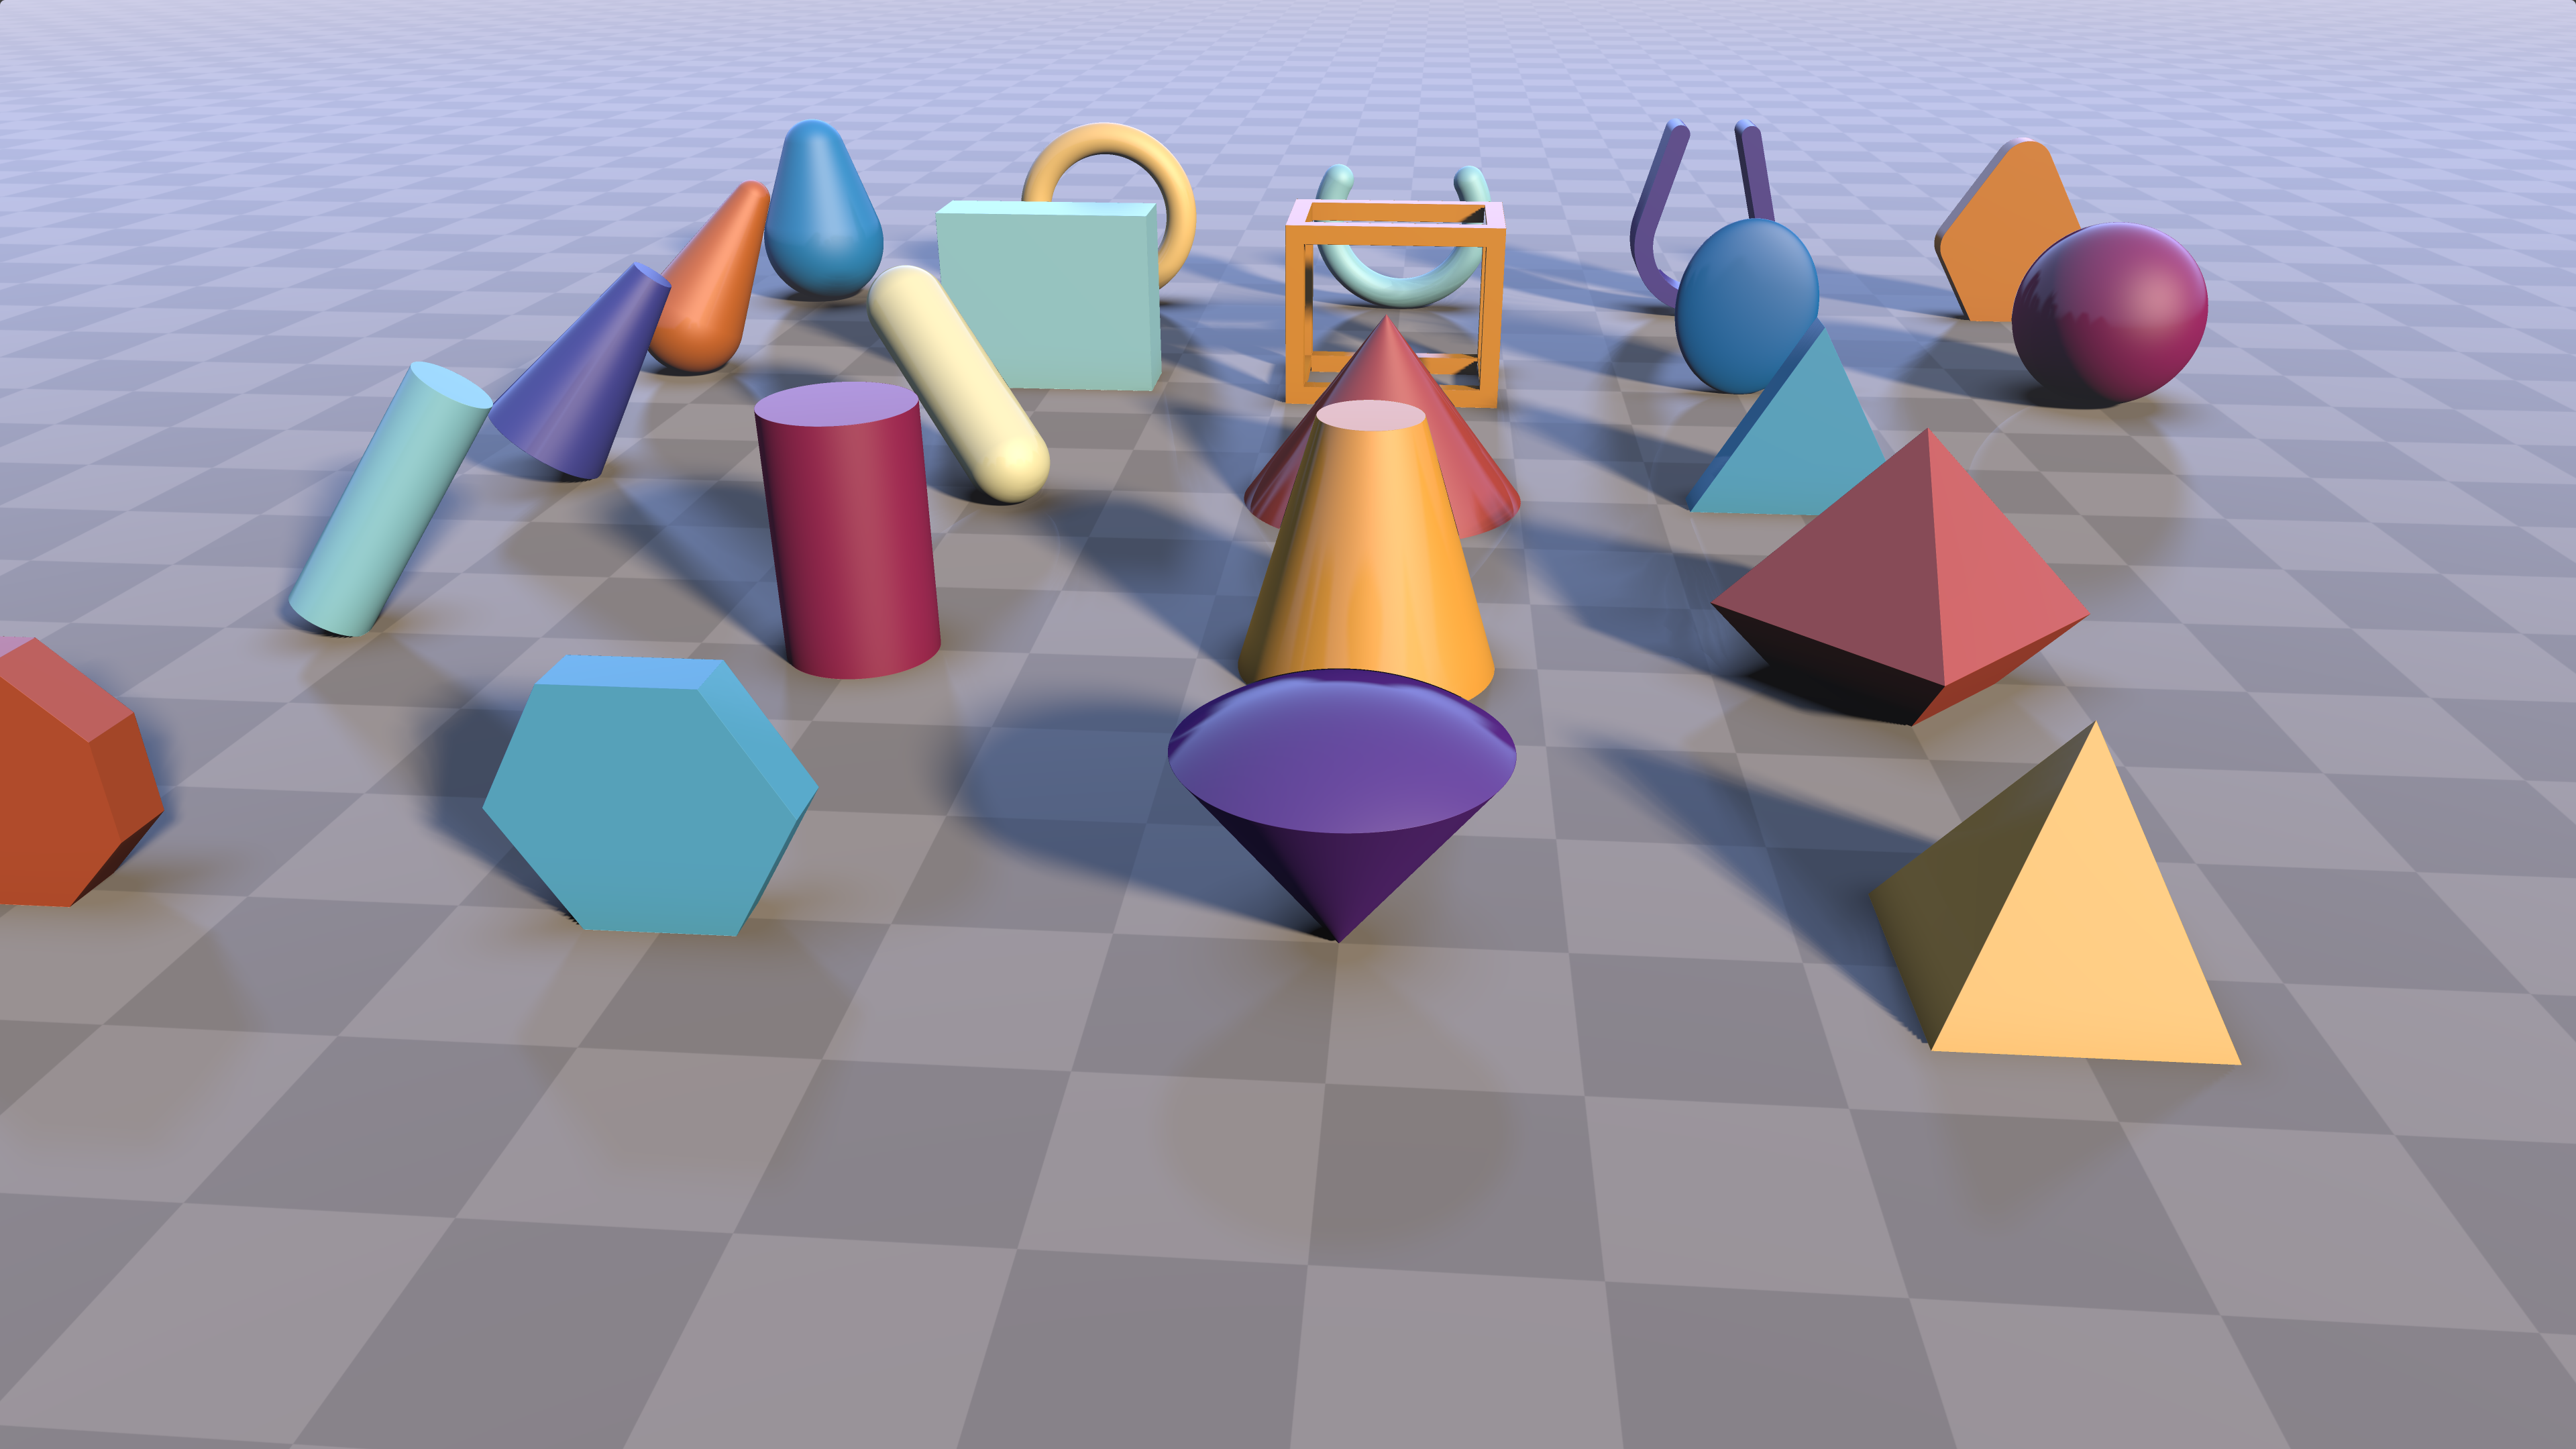
\includegraphics[width=\textwidth]{img/Demo/Raymarching-Primitives}
   \caption{\href{https://www.shadertoy.com/view/Xds3zN}{Raymarch Primitives}}
 \end{subfigure}
~
 \begin{subfigure}[b]{0.42\textwidth}
   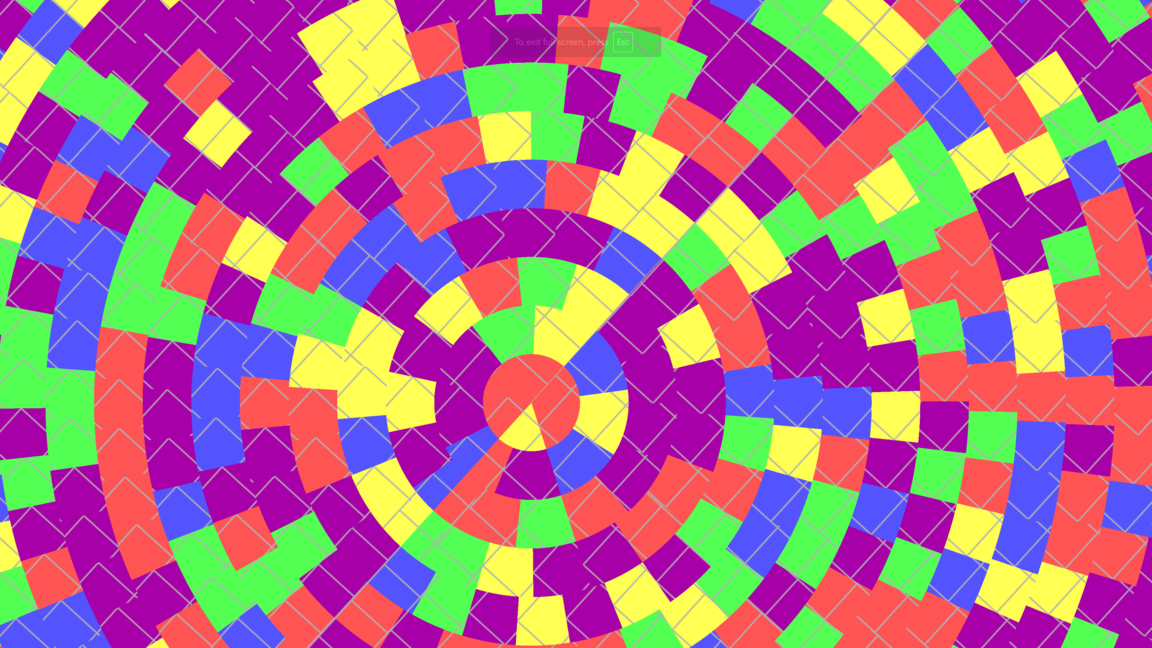
\includegraphics[width=\textwidth]{img/Demo/AnimatedCentricMosaicTiles}
   \caption{\href{https://www.shadertoy.com/view/43tfRr}{Centric Mosaic Tiles}}
 \end{subfigure}
 \caption{Propiedad de los respectivos autores.}
\end{figure}
\end{columns}
\end{frame}

\begin{frame}{¿Qué \emph{no es} éste taller?}
    No es un curso \emph{completo} de \say{Graficación por Computadora}.
    Mas aun, no vamos a enseñar a hacer gráficas por computadora de manera correcta.
    \begin{itemize}
         \item Usar este paradigma \alert{es un juego}. No se usa en producción.
         \item Los shaders que vamos a escribir son ineficientes.
         \item El código puede ser ofuscado.
     \end{itemize}
     Por razones de tiempo, tampoco enseñaremos todo lo que hay en el truco.
     \begin{block}{}
         \begin{itemize}
            \item Este es un taller \alert{básico} de shaders de juguete (Shadertoy).
            \item Revisaremos un conjunto de técnicas simples.
            \item Recuerda: hacer shaders complejos, requiere de experiencia, creatividad y tiempo.
        \end{itemize}  
    \end{block}
\end{frame}

\begin{frame}{¿Qué puedo aprovechar de éste taller?}
    \begin{itemize}
         \item Aprender una manera de expresión artística usando programación.
         \item Un excelente ejercicio para fomentar la creatividad.
         \item Una forma de practicar, aplicar y mejorar tus conocimientos de matemáticas y de computación.
         \item Un medio de compartir con una comunidad (Shadertoy tiene elementos de red social).
         \item Se convierte en un hobby productivo.
     \end{itemize}
     
     \begin{block}{Graficación por Computadora}
         \begin{itemize}
            \item Una probadita para saber si estas interesado en tomar un curso formal después.
            \item Si ya tomaste el curso, es un \emph{hack} muy elegante que seguramente no se te había ocurrido.
            \item Muchos profesionales del área lo practican como hobby.
        \end{itemize}  
    \end{block}
\end{frame}

\begin{frame}{Acerca de mí}
    \begin{columns}
\column[t]{0.5\textwidth}
        \begin{figure}[htb]
            \centering
            
\includegraphics[width=0.6\textwidth]{img/Avatar12}
            \caption{Dr. Jorge Antonio García Galicia.}
        \end{figure}
\column[t]{0.5\textwidth}
     \begin{itemize}
         \item \href{https://mac.acatlan.unam.mx/}{Licenciatura} y \href{https://www.pcic.unam.mx/}{maestría} en la \href{https://www.unam.mx/}{UNAM}.
         \item \href{https://polytechnic.purdue.edu/degrees/phd-technology}{Doctorado} en \href{https://www.purdue.edu/}{Purdue University}.
         \item Hice una pasantía en \href{https://research.adobe.com/}{Adobe} y trabajé en \href{https://www.nvidia.com/}{Nvidia}.
         \item He dado clases en \href{https://www.acatlan.unam.mx/}{Acatlán} y fui ayudante en \href{https://www.fciencias.unam.mx/directorio/63922}{Ciencias} y en \href{https://polytechnic.purdue.edu/}{Purdue}.
         \item Actualmente soy SWE en \href{https://about.google/}{Google}.
         \item Tengo mas de 15 años de experiencia en Tecnología.
     \end{itemize}
\end{columns}
\end{frame}

\begin{frame}{Mi experiencia con gráficos}
\begin{columns}
\column[t]{0.5\textwidth}
    \begin{itemize}
         \item Tres tesis que tienen que ver con \href{https://en.wikipedia.org/wiki/Computer_graphics}{Graficación por Computadora}.
         \item Publicado en \href{https://direct.mit.edu/leon}{Leonardo}, \href{https://www.siggraph.org/}{SIGGRAPH} y en \href{https://www.eg.org/wp/eurographics-publications/}{Eurographics}.
         \item Trabajé en el driver de \href{https://www.opengl.org/}{OpenGL} y en \href{https://stadia.google.com/gg/}{Stadia}.
         \item Actualmente trabajo en \href{https://www.android.com/xr/}{AndroidXR}.
         \item Provengo de una familia de artistas.
     \end{itemize}
\column[t]{0.5\textwidth}
\begin{figure}[htp]
 \centering
 \begin{subfigure}[b]{0.4\textwidth}
   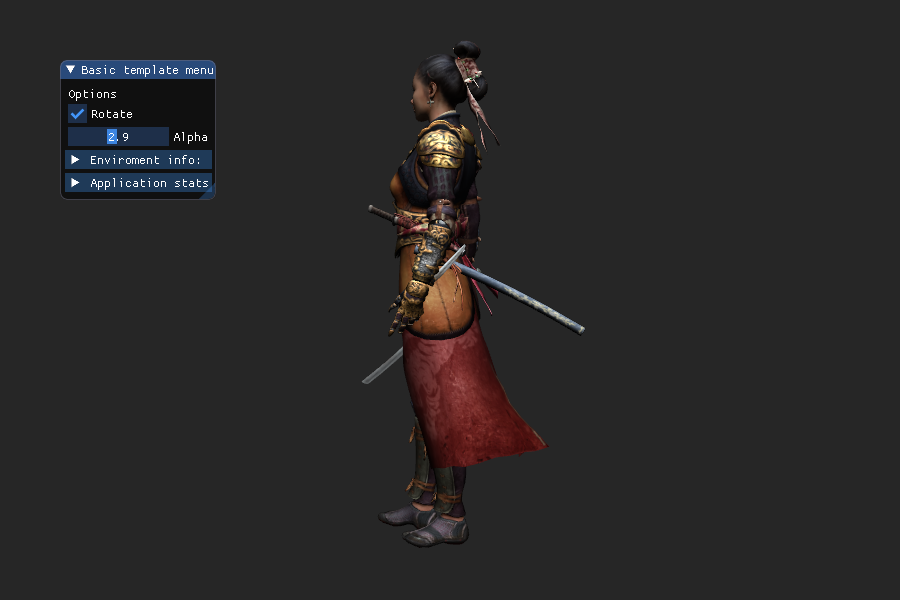
\includegraphics[width=\textwidth]{img/menuTemplate}
 \end{subfigure}
~
 \begin{subfigure}[b]{0.4\textwidth}
   
\includegraphics[width=\textwidth]{img/completo}
 \end{subfigure}
\\
 \begin{subfigure}[b]{0.4\textwidth}
   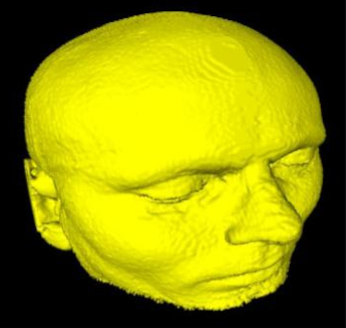
\includegraphics[width=\textwidth]{img/master}
 \end{subfigure}
~
\begin{subfigure}[b]{0.4\textwidth}
   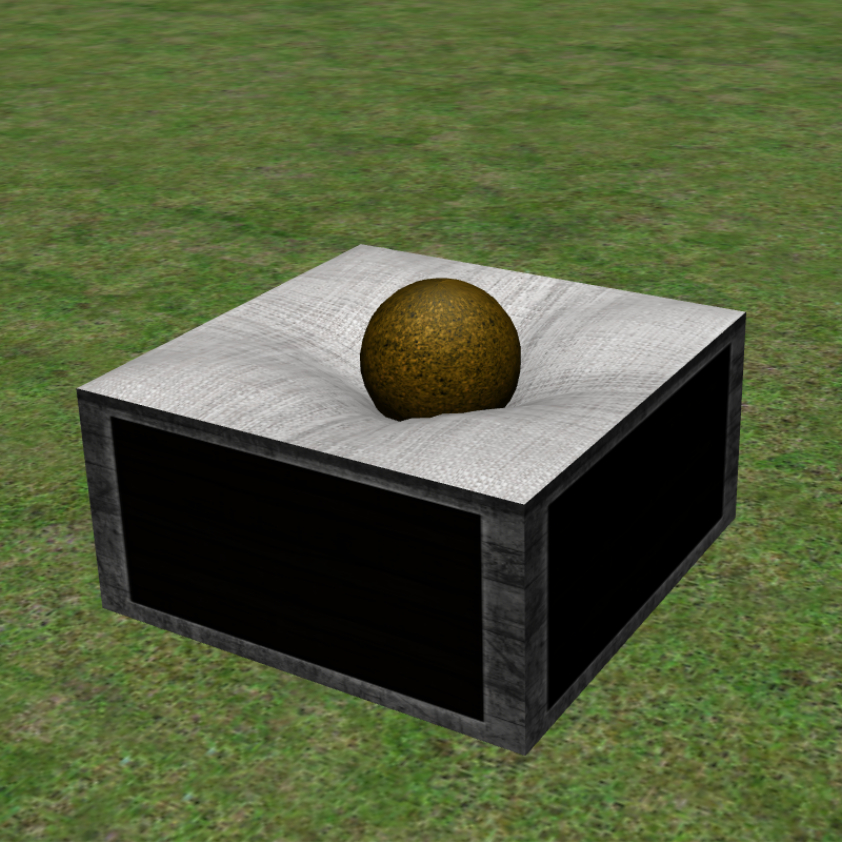
\includegraphics[width=\textwidth]{img/bachelor_thesis}
 \end{subfigure}
 
\end{figure}
\end{columns}
\end{frame}

\section{Gráficas por computadora actualmente}

\begin{frame}{El GPU}
\begin{block}{Graphics processing unit (GPU)}
    Un procesador programable con alta capacidad de computo en paralelo, que generalmente opera con imágenes digitales.
\end{block}
    \begin{itemize}
        \item Originalmente estaba dedicado a hacer gráficos.
        \item Actualmente, hace computo general, de hecho es el \href{https://en.wikipedia.org/wiki/AI_accelerator}{AI acelerator} mas usado.
        \item No confundir con una tarjeta de video: Todas la tarjetas de video (actuales) tiene un GPU. Pero no todos los GPU están en tarjetas de video.
        \item Cuando un GPU esta físicamente separado del chip que tiene el CPU se le llama un GPU discreto.
     \end{itemize}
\end{frame}

\begin{frame}{¿Qué es un shader?}
\begin{block}{Shader}
    Un programa que es ejecutado de manera paralela en el GPU como parte de un pipeline.
\end{block}
Acerca del nombre:
    \begin{itemize}
        \item El termino fue acuñado por Pixar en 1988 para Renderman.
        \item Originalmente (2001), los shaders solo hacían cálculos de iluminación: intensidad de la luz, color, sombras y brillos.
        \item De ahí su nombre, que significa \emph{sombreado}.
     \end{itemize}

\end{frame}

\begin{frame}{La pieza básica}
\begin{block}{Pipeline gráfico.}
    Es una abstracción de SW, que describe el proceso que debe seguir un programa para trasformar una escena tridimensional en una imagen.
\end{block}
\begin{figure}[htb]
  \centering
  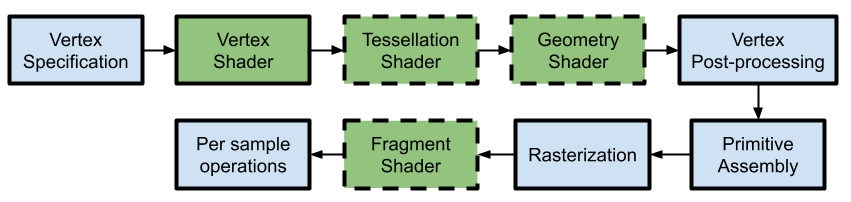
\includegraphics[width=0.7\textwidth]{img/RenderPipeline}
\end{figure} 
\end{frame}

\begin{frame}{Simplificando\ldots}
\begin{itemize}
    \item El la práctica, los tesselation shaders y los geometry shaders solo se usan para cosas muy especificas.
    \item Mas aún, casi nunca se configuran los estados entre el vertex shader y la rasterización.
    \item Para propósitos de esta explicación, podemos pensarlo de manera mas simple:    
\end{itemize}
\begin{figure}[htb]
  \centering
  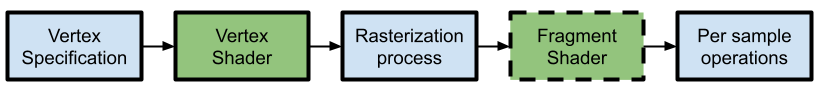
\includegraphics[width=0.7\textwidth]{img/SimplifiedPipeline}
\end{figure}
\end{frame}

\begin{frame}[allowframebreaks]{¿Cómo se programa una aplicación gráfica?}
\begin{itemize}
    \item En general tienes que usar al menos tres cosas:
    \begin{enumerate}
        \item Un lenguaje de programación en el CPU para crear una aplicación.
        \item Un API gráfico, para construir, configurar y conectar el pipeline.
        \item Un lenguaje para escribir shaders.
    \end{enumerate}
    \item En este taller solo escribiremos código de shaders usando \href{https://www.khronos.org/opengl/wiki/OpenGL_Shading_Language}{GLSL}.
    \item Pero sin darnos cuenta el navegador de hecho usa: \href{https://en.wikipedia.org/wiki/JavaScript}{javascript} y \href{https://www.khronos.org/webgl/}{WebGL}, que es un \href{https://www.khronos.org/opengles/}{subconjunto de OpenGL}.
\end{itemize}
\begin{figure}[htb]
  \centering
  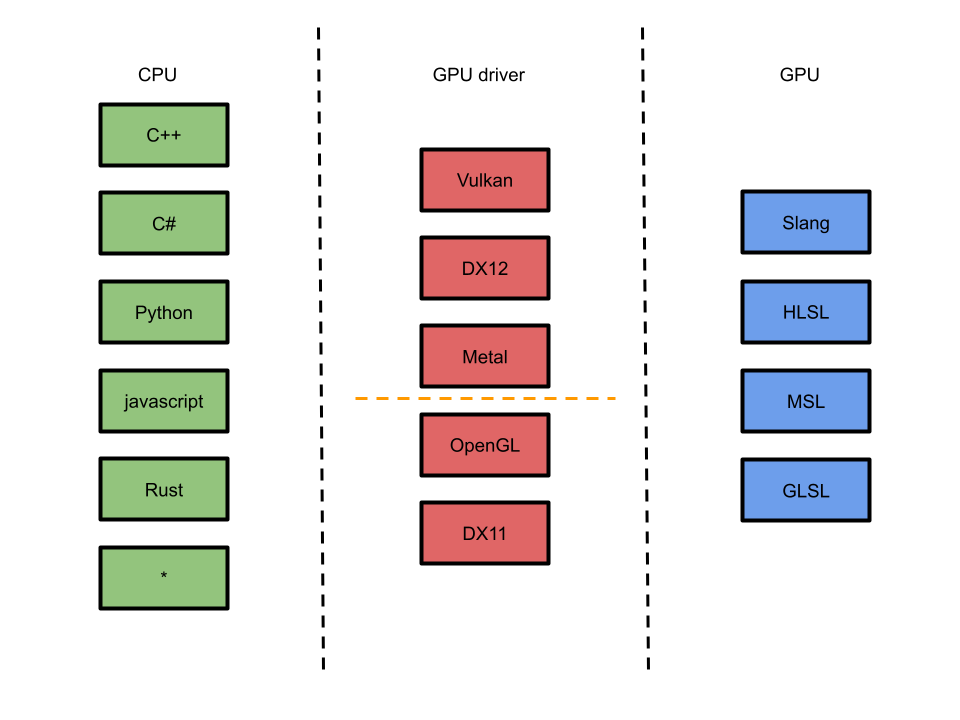
\includegraphics[width=0.6\textwidth]{img/APIs}
  %\caption{Hay varias opciones para cada caso}
\end{figure}
\end{frame}

\begin{frame}[allowframebreaks]{Anatomía de una aplicación}
Actualmente, una aplicación típica:
    \begin{itemize}
        \item Esta escrita en un engine gráfico (Como \href{https://unity.com/}{Unity} o \href{https://www.unrealengine.com/}{Unreal}).
        \item Para producir un frame, se usan cientos de pipelines.
        \begin{itemize}
            \item Varios pipelines, producen resultados en texturas que luego otros pipelines consumen.
            \item Cada material de los objetos de la escena tiene su propio pipeline.
            \item Hay pipelines especializados en ciertas tareas (Sombras, reflexiones, iluminación, etc.).
            \item Algunos son directos, otros diferidos, otros por mosaicos.
            \item Sin contar que muchos efectos se llevan a cabo en compute shaders.
        \end{itemize}
    \end{itemize}
    \begin{figure}[htb]
        \centering
        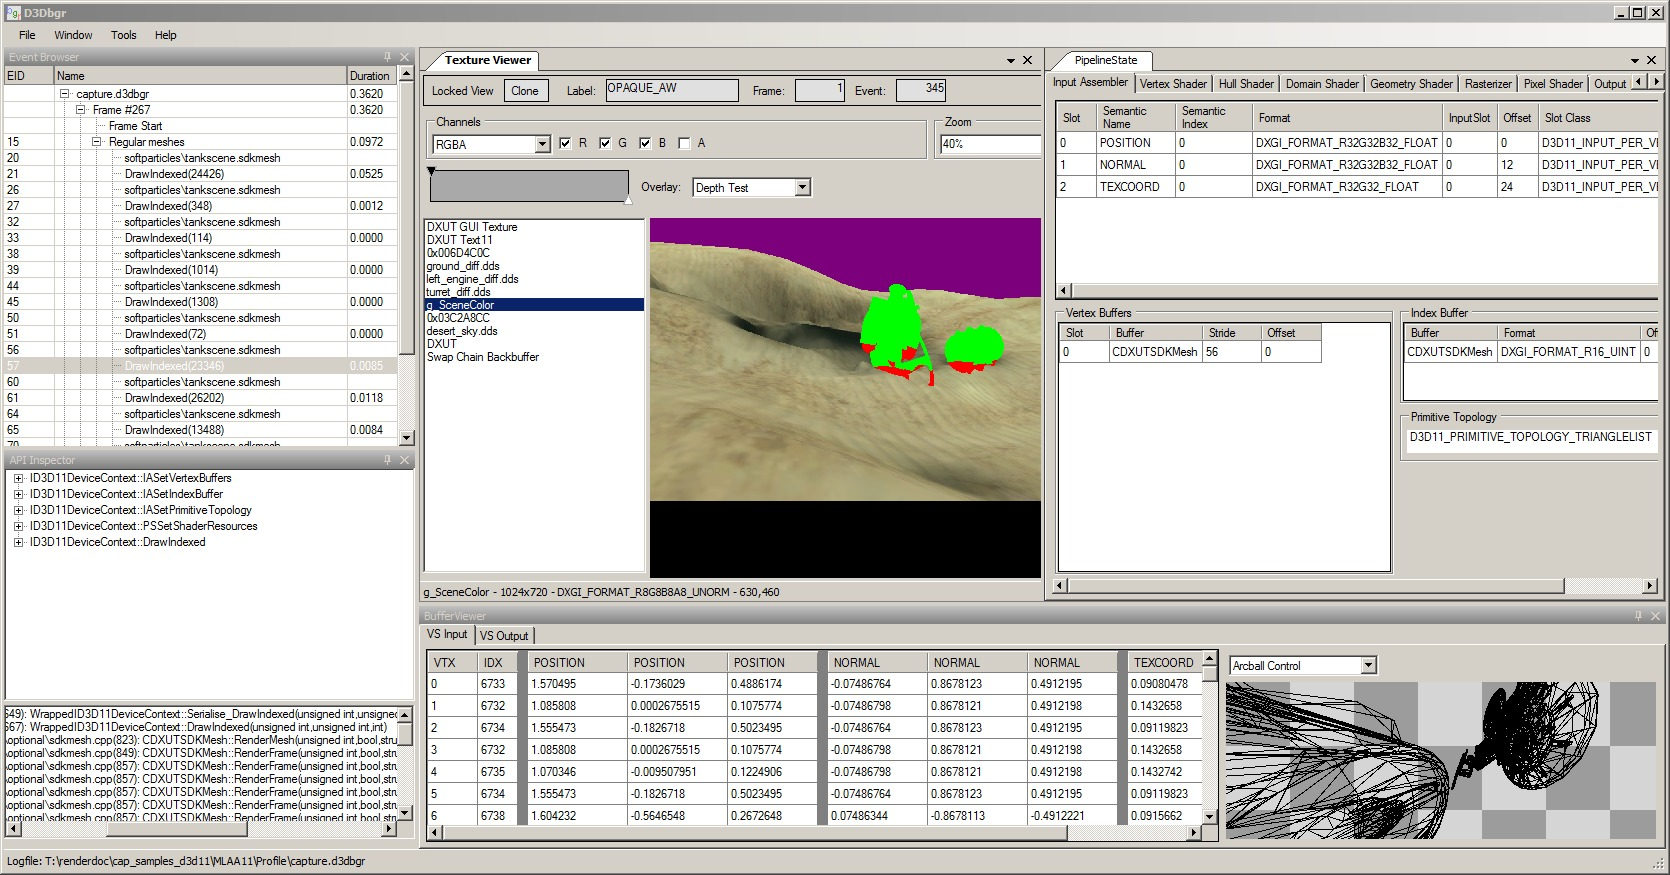
\includegraphics[width=0.8\textwidth]{img/functionality}
    \end{figure}
\end{frame}

\begin{frame}{¿Qué nos depara el futuro?}
\begin{columns}
\column[t]{0.5\textwidth}
    Hay una tendencia importante hacia:
    \begin{itemize}
        \item Unificar en el modelo de \href{https://en.wikipedia.org/wiki/Physically_based_rendering}{iluminación PBR}.
        \item Las técnicas basadas en rayos: \href{https://en.wikipedia.org/wiki/Path_tracing}{Pathtracers}.
        \begin{itemize}
            \item Generar parte de los fragments de un frame (o incluso frames completos), \href{https://www.youtube.com/watch?v=5PHBXY0FI5o&t=2s}{usando técnicas de AI} en vez de calcularlos.
        \end{itemize}
        \item Definir un nuevo pipeline: Task (Amplification) shaders, \href{https://www.khronos.org/blog/mesh-shading-for-vulkan}{Mesh shaders}.
        \item Descargar la mayor parte de las tareas en el \href{https://en.wikipedia.org/wiki/Compute_kernel}{Compute shader}.
    \end{itemize}
\column[t]{0.5\textwidth}
\begin{figure}[htp]
  \centering
  \includegraphics[width=0.6\textwidth]{img/pathtracer}
\end{figure}
\end{columns}
\end{frame}


\section{Shadertoy}

\begin{frame}{Una idea ingeniosa}
Todo empezó con una \href{https://iquilezles.org/articles/nvscene2008/rwwtt.pdf}{plática}: \say{Rendering Worlds With Two Triangles} presentada en la \href{https://www.youtube.com/watch?v=A1iW6Z_Jc4k}{conferencia NVScene} el 22 Aug 2008 por \href{https://iquilezles.org/}{Iñigo Quilez}
\begin{exampleblock}{}
\begin{enumerate}
    \item Si dibujamos un cuadrado (formado por 2 triángulos), que cubre toda la ventana. Esto provocará la ejecución del fragment (pixel) shader en todos los píxeles de la pantalla. 
    \item Luego, usamos el fragment shader en donde cada fragment (pixel) sabe su respectiva posición en el render target, unas constantes (uniforms) y un montón de matemáticas, para dibujar la escena.
\end{enumerate}
\end{exampleblock}
\begin{figure}[htp]
  \centering
  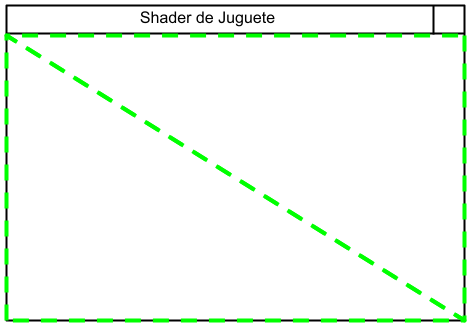
\includegraphics[width=0.2\textwidth]{img/TwoTriangles}
\end{figure}
\end{frame}

\begin{frame}{Regresar al principio}
\begin{figure}[htp]
  \centering
  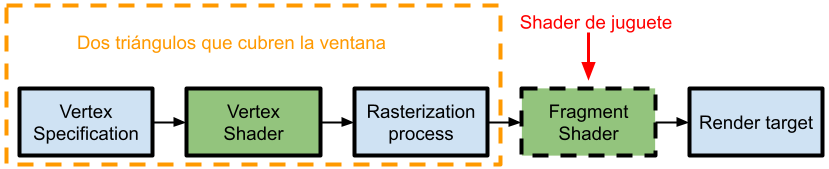
\includegraphics[width=0.7\textwidth]{img/Truco}
\end{figure}
\begin{itemize}
    \item Es similar a como se hacían los gráficos antes de que tuviéramos tarjetas de video.
    \item Solo que ahora aprovechamos el \alert{inmenso poder paralelo} del GPU
    \item Y usamos GLSL
\end{itemize}
\end{frame}

\begin{frame}{Nota curiosa}
\begin{figure}[htp]
  \centering
  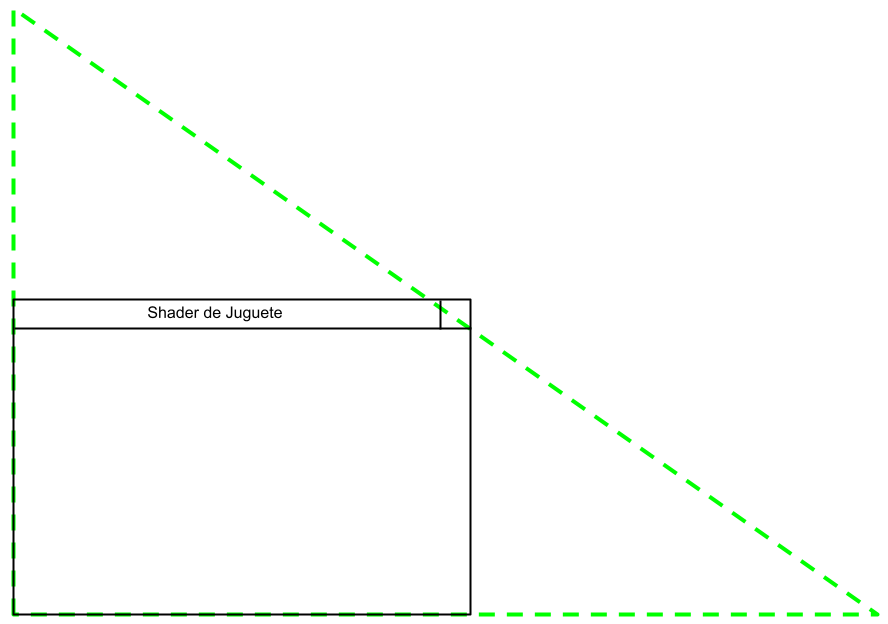
\includegraphics[width=0.4\textwidth]{img/onetriangle}
\end{figure}
De hecho podemos hacerlo con un solo triángulo y luego hacemos clipping.
\end{frame}

\begin{frame}{Actualmente, es mejor hacer:}
\begin{figure}[htp]
  \centering
  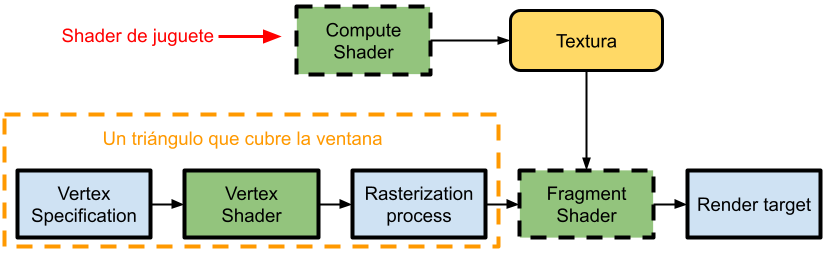
\includegraphics[width=0.65\textwidth]{img/TrucoModerno}
\end{figure}
\end{frame}

\begin{frame}{Shadertoy}
\begin{itemize}
    \item Shadertoy es un sitio web: \url{https://www.shadertoy.com/} que nos da la infraestructura para usar el truco
    \item Y ciertas herramientas sociales
    \item Fue creado por \href{https://iquilezles.org/}{Iñigo Quilez} y \href{https://www.poljeremias.com/}{Pol Jeremias} en el 2013
\end{itemize}
\begin{figure}[htp]
  \centering
  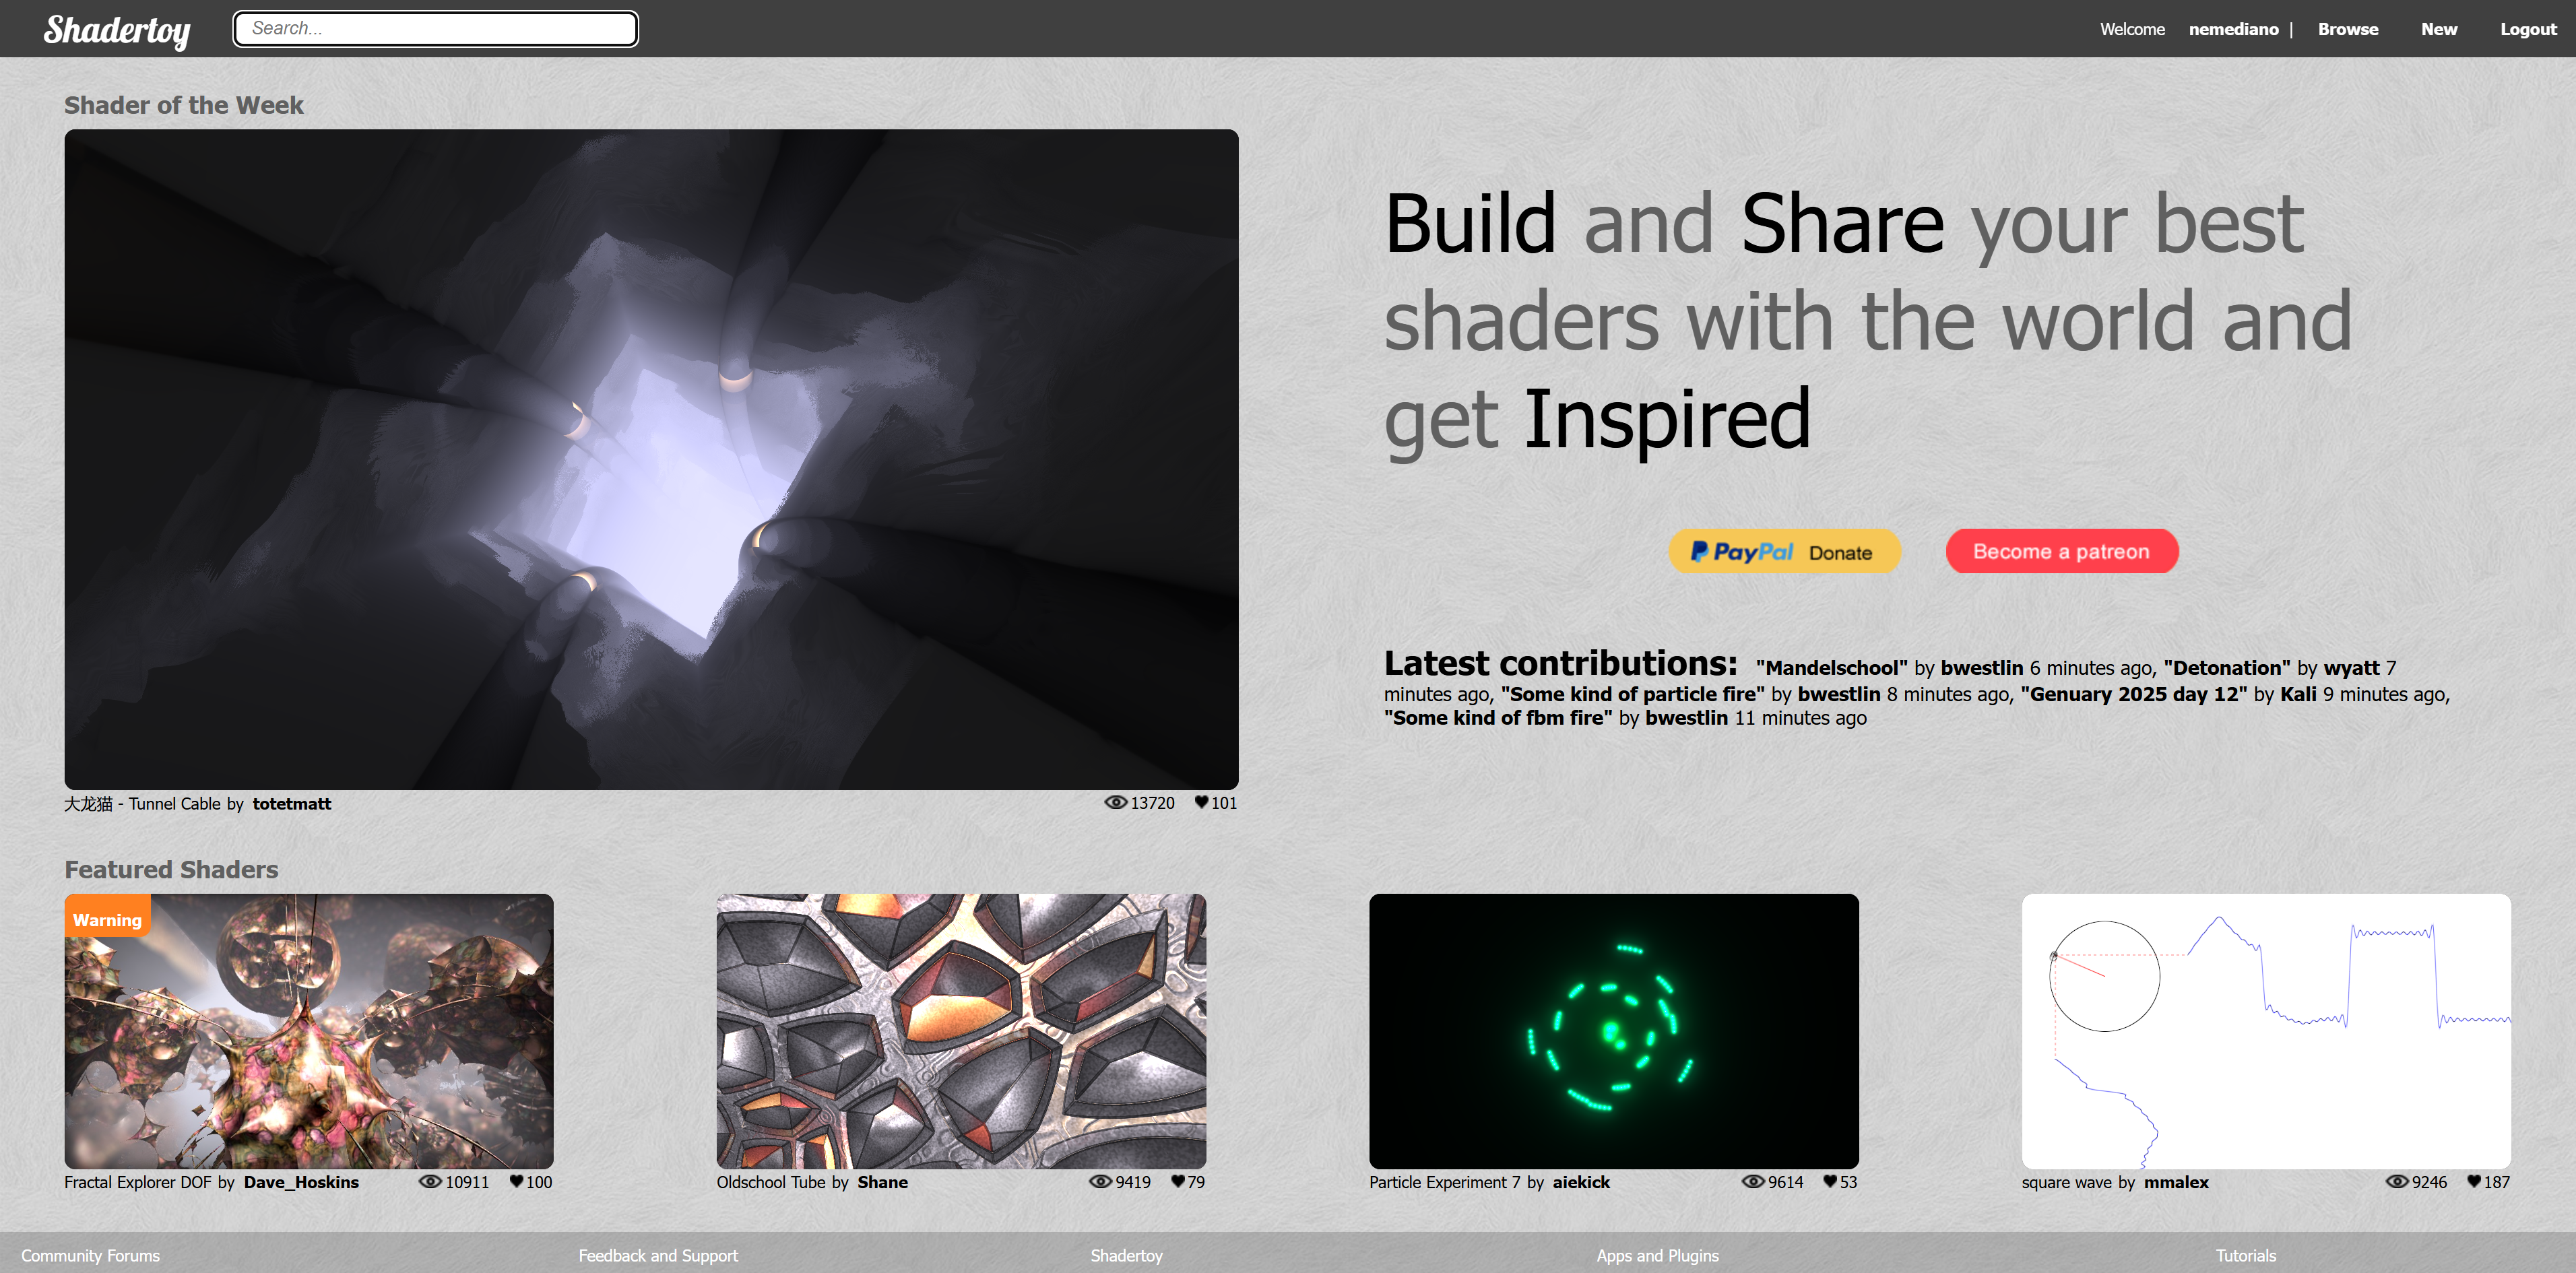
\includegraphics[width=0.4\textwidth]{img/ShaderToySite}
\end{figure}
\end{frame}

\begin{frame}{¿Cómo se usa?}
Escribir un programa en \href{https://www.khronos.org/opengl/wiki/Core_Language_(GLSL)}{GLSL} que se ejecuta en paralelo por cada pixel de la salida.
\begin{itemize}
    \item \textbf{Entradas:} recibes la coordenada del pixel
    \item \textbf{Salida:} debes regresar el color del pixel
    \item Recibe algunas constantes extra: el tiempo, el tamaño total del render target, etc.
\end{itemize}
\begin{figure}[htp]
  \centering
  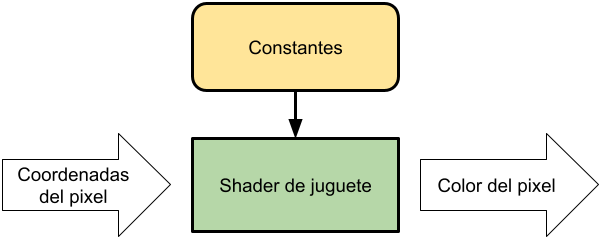
\includegraphics[width=0.4\textwidth]{img/SimpleShaderToy}
\end{figure}
\end{frame}

\begin{frame}{Así se ve}
\begin{figure}[htp]
  \centering
  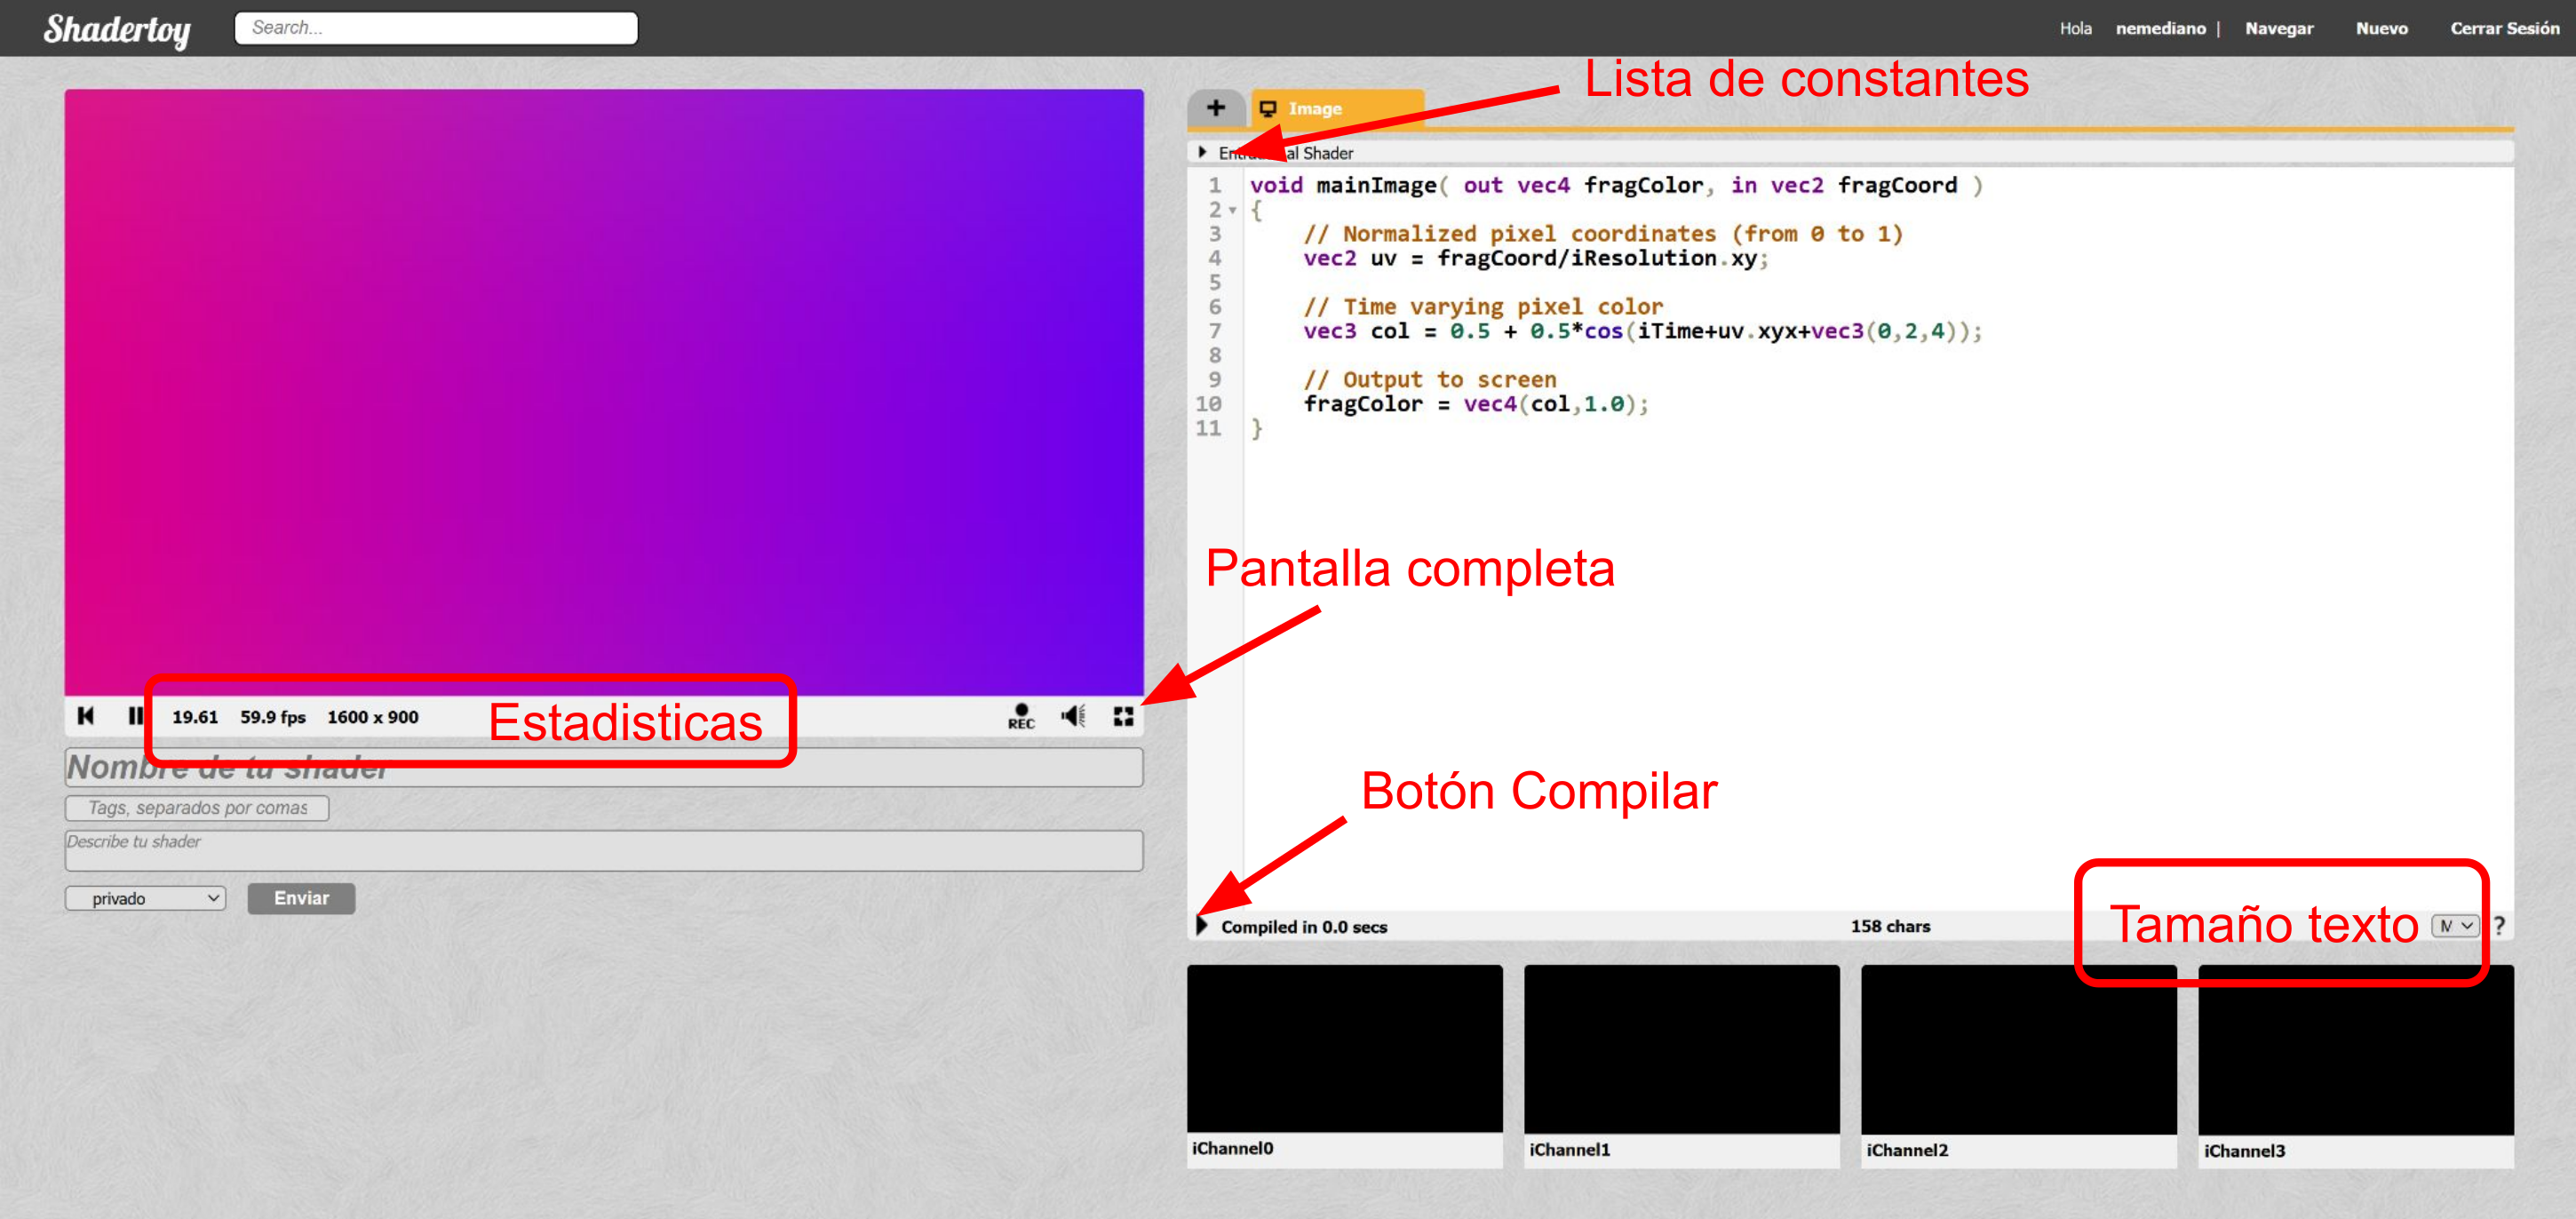
\includegraphics[width=0.8\textwidth]{img/ShaderToyUI}
\end{figure}
\end{frame}

\begin{frame}{Portabilidad}
Shadertoy:
\begin{itemize}
    \item Crea el pipeline por nosotros
    \item Inyecta código en el fragment shader
\end{itemize}
Pero ten por seguro que:
\begin{block}{}
    Cualquier shader que funciona en shadertoy, puede ser \alert{portado} y funcionar en cualquier otro entorno que pueda desplegar gráficos.
\end{block}
Adicionalmente:
\begin{itemize}{}
    \item Hay muchos entornos de programación, que emulan Shadertoy
    \item Siempre puedes escribir tu propio programa que ejecute shaders de shadertoy
\end{itemize}
\begin{block}{}
    No es tan difícil, cualquier alumno que haya tomado una clase de CG puede hacerlo fácilmente.
\end{block}
\end{frame}

\section{GLSL: Lenguaje para escribir shaders}

\begin{frame}[fragile]{Tipos primitivos}
Esta \alert{no es} una lista exhaustiva, ante la duda consulta la \href{https://www.khronos.org/opengl/wiki/Data_Type_(GLSL)}{referencia}.
\begin{itemize}
    \item Tipos de escalares: \mintinline{glsl}{float}, \mintinline{glsl}{int}, \mintinline{glsl}{bool}.
    \item Vectores de $n \in \{2, 3, 4\}$ dimensiones: \mintinline{glsl}{vec3}, \mintinline{glsl}{ivec2}, \mintinline{glsl}{bvec4}.
    \begin{itemize}
        \item Nótese que cuando el tipo subyacente es \mintinline{glsl}{float} no se requiere el prefijo.
    \end{itemize}
    \item Los operadores aritméticos entre vectores se aplican por componente.
    \begin{itemize}
        \item Requieren que los operandos sean del mismo tamaño
    \end{itemize}
    \item Matrices de $n\times m$ dimensiones donde $n, m \in \{2, 3, 4\}$ dimensiones: \mintinline{glsl}{mat2x3}, \mintinline{glsl}{mat3x4}.
    \begin{itemize}
        \item Todas las matrices son de tipo \mintinline{glsl}{float}
        \item Las matrices cuadradas se pueden abreviar: \mintinline{glsl}{mat2}
        \item Las operaciones entre matrices, son las esperadas del álgebra lineal
    \end{itemize}
    \item Las multiplicaciones: \say{matriz por matriz}, \say{matriz por vector}, \say{escalar por vector} y  \say{escalar por matriz} son las definida en álgebra lineal.
\end{itemize}

\end{frame}

\begin{frame}[fragile]{Swizzling}
\begin{itemize}
    \item Los tipos vectoriales tienen accesores y mutadores a sus componentes individuales.
    \item Los accesores tienen tres sintaxis equivalentes: $(x, y, z, w), (r, g, b, a), (s, t, p, q)$.
\end{itemize}
Esto define el llamado Swizzling:
\begin{listing}
\begin{minted}{glsl}
vec2 someVec;
vec4 otherVec = someVec.xyxx;
vec3 thirdVec = otherVec.zyy;
vec4 fourthVec;
// Tambien funciona en l-values:
fourthVec.wzyx = vec4(1.0, 2.0, 3.0, 4.0); // Reverses the order.
fourthVec.zx = vec2(3.0, 5.0); // Sets the 3rd component to 3 and the 1st component to 5
\end{minted}
\end{listing}
\end{frame}

\begin{frame}[fragile]{Constructores de vectores}
Se pueden construir a partir de:
\begin{itemize}
    \item Vectores de mayor dimensión (los componentes extra son ignorados).
    \item Una combinación de escalares y de vectores de menor dimensión.
    \item De manera abreviada, especificando un solo escalar que se repite.
\end{itemize}
\begin{listing}
\begin{minted}{glsl}
vec4(vec2(10.0, 11.0), 1.0, 3.5) == vec4(10.0, vec2(11.0, 1.0), 3.5);
vec3(vec4(1.0, 2.0, 3.0, 4.0)) == vec3(1.0, 2.0, 3.0);
vec4(vec3(1.0, 2.0, 3.0)); // error. Not enough components.
vec2(vec3(1.0, 2.0, 3.0)); // OK
vec3(1.0) // Abreviation to say: vec3(1.0, 1.0, 1.0);
\end{minted}
\end{listing}
\end{frame}


\begin{frame}[fragile]{Constructores de matrices}
\begin{itemize}
    \item Se construyen por columnas.
    \item Se pueden construir a partir de matrices de menor o igual dimensión.
    \item O de manera abreviada especificando un solo escalar que llena la diagonal.
\end{itemize}
\begin{listing}
\begin{minted}{glsl}
mat2(
  float, float,   // first column
  float, float);  // second column

mat4(
  vec4,           // first column
  vec4,           // second column
  vec4,           // third column
  vec4);          // fourth column

mat3 diagMatrix = mat3(5.0);  // Diagonal matrix with 5.0 on the diagonal.
mat4 otherMatrix = mat4(diagMatrix); // The last element on the diagonal is 1.0
\end{minted}
\end{listing}
\end{frame}

\begin{frame}{Built-in functions}
Además de las funciones habituales esperadas, algunas funciones interesantes:
\begin{table}[htb]
  \begin{center}
    \begin{tabular}{l | l }
      \mintinline{glsl}{vec3 mix(vec3 x, vec3 y, float a)} & Interpolación lineal \\
      \mintinline{glsl}{vec3 step(float edge, vec3 x)} & Función escalón \\
      \mintinline{glsl}{mat4 inverse(mat4 M)} & Matriz inversa \\
      \mintinline{glsl}{float dot(vec3 x, vec3 y)} & Producto punto \\
      \mintinline{glsl}{vec3 cross(vec3 x, vec3 y)} & Producto cruz \\
      \mintinline{glsl}{vec3 reflect(vec3 i, vec3 n)} & Reflejar $\mathbf{i}$ a partir de $\mathbf{n}$ \\
      \mintinline{glsl}{vec3 clamp(vec3 x, vec3 min, vec3 max)} & Limitar entre dos valores \\
      \mintinline{glsl}{float length(vec3 x)} & Norma de un vector \\
      \mintinline{glsl}{vec3 normalize(vec3 x)} & Vector normalizado \\
      \mintinline{glsl}{float distance(vec3 x, vec3 y)} & Distancia entre dos puntos \\
    \end{tabular}
  \end{center}
\end{table}
Todas las funciones tienen las sobrecargas vectoriales, cuando corresponde.
\end{frame}

\section{Mis primeros shader de juguete}
\begin{frame}{Repositorio}
Todo lo necesario para este taller esta en este repositorio: 
\begin{block}{}
\url{https://github.com/nemediano/tallerShadertoy}.
\end{block}
\begin{itemize}
    \item Ésta presentación, también esta en el mismo repositorio. Así puedes seguir los links.
    \item Para cada ejercicio, hay dos versiones de código fuente.
    \begin{enumerate}
        \item El código mínimo para empezar el ejercicio
        \item Una posible solución al ejercicio 
    \end{enumerate}
\end{itemize}

\end{frame}

\begin{frame}{Últimos detalles}
En shadertoy, la ejecución inicia y termina con la función:

\mintinline{glsl}{void mainImage(out vec4 fragColor, in vec2 fragCoord)}.

\begin{itemize}
    \item Por cada fragment recibes de parámetro: \mintinline{glsl}{fragCoord}, con la posición del fragment en el \emph{render target}.
    \item La salida: \mintinline{glsl}{fragColor}, es un output parameter. Un vector de dimensión 4 que debe contener el color final del fragment.
    \begin{itemize}
        \item La salida $\mathbf{x} \in \mathbb{R}^{4}$ debe tener $ x_i \in [0, 1]$.
        \item El último componente $x_4$ (ó bien $w$), representa el componente alpha, que en Shadertoy debe ser 1.
    \end{itemize}
\end{itemize}
\end{frame}

\begin{frame}{Ejercicio: Bandera a cuadros}
    \begin{columns}
\column[t]{0.5\textwidth}
     \begin{itemize}
         \item Tratar de escribir un shader que genere una bandera a cuadros (o tablero de ajedrez si lo prefieres)
         \item Puedes empezar con el código de default de shader toy.
         \item Recuerda las funciones trigonométricas
     \end{itemize}
\column[t]{0.5\textwidth}
        \begin{figure}[htb]
            \centering
            
\includegraphics[width=0.6\textwidth]{img/Ejer1}
            \caption{\url{https://github.com/nemediano}}
        \end{figure}
\end{columns}
\end{frame}


\subsection{Funciones de distancia}

\begin{frame}{Sistema de coordenadas}
\begin{columns}
\column[t]{0.5\textwidth}
    \begin{itemize}
         \item Al principio, las coordenadas del fragment están en el espacio del imagen del render target. Miden pixeles.
         \item Cuando dividimos entre la resolución del render target, están en coordenadas de textura ($uv$-mapping). $u,v \in [ 0,1 ]$
     \end{itemize}
\column[t]{0.5\textwidth}
\begin{figure}[htp]
 \centering
 \begin{subfigure}[b]{0.45\textwidth}
   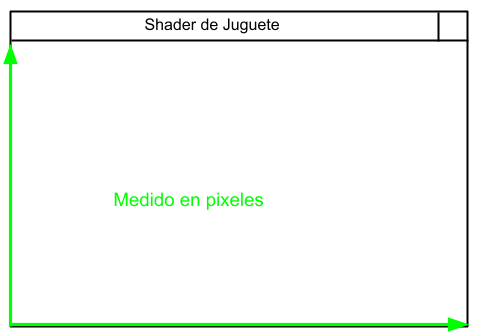
\includegraphics[width=\textwidth]{img/FrameOfreference}
   \caption{Espacio de imagen}
 \end{subfigure}
\\
 \begin{subfigure}[b]{0.45\textwidth}
   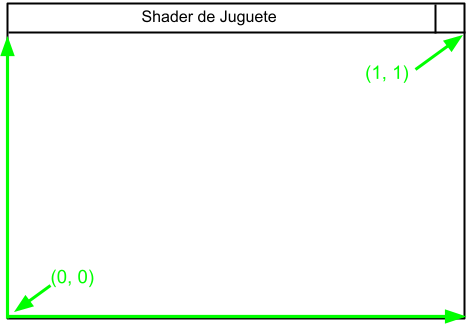
\includegraphics[width=\textwidth]{img/FoRUVSpace}
   \caption{$uv$ space}
 \end{subfigure}
\end{figure}
\end{columns}
\end{frame}

\begin{frame}{Sistema de coordenadas II}
\begin{columns}
\column[t]{0.5\textwidth}
    \begin{itemize}
        \item Cuando restamos 0.5 y multiplicamos por dos. Están en coordenadas normalizadas. $x,y \in [-1, 1]$.
        \item Cuando corregimos con el \emph{aspect ratio} de la pantalla, están en coordenadas de la escena. El origen esta en el centro, el eje mas restrictivo esta en $[-1, 1]$ y el otro es proporcional.
     \end{itemize}
\column[t]{0.5\textwidth}
\begin{figure}[htp]
 \centering
 \begin{subfigure}[b]{0.45\textwidth}
   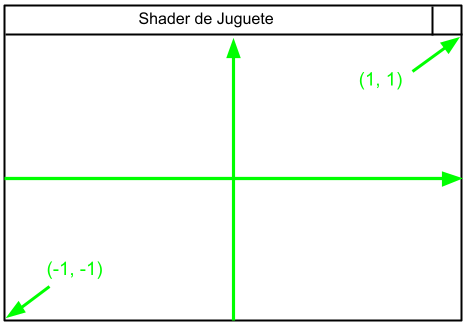
\includegraphics[width=\textwidth]{img/FoRNormalized}
   \caption{Normalize coordinates}
 \end{subfigure}
\\
 \begin{subfigure}[b]{0.45\textwidth}
   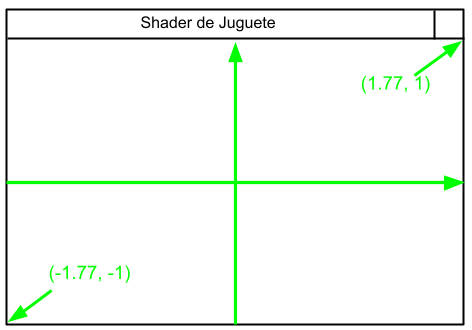
\includegraphics[width=\textwidth]{img/FoRCorrected}
   \caption{World Coordinates}
 \end{subfigure}
\end{figure}
\end{columns}
\end{frame}

\begin{frame}[fragile]{Función de transformación}
\begin{listing}
\begin{minted}{glsl}
vec3 getWorldCoordinates(vec2 fragCoord, vec3 iResolution) {

    float aspectRatio = iResolution.x / iResolution.y;

    vec2 scaleFactor =
        iResolution.x > iResolution.y ? vec2(aspectRatio, 1.0) : vec2(1.0, 1.0 / aspectRatio);

    vec2 world = scaleFactor * (2.0 * (fragCoord/iResolution.xy) - vec2(1.0));

    return vec3(world, 1.0);
}
\end{minted}
\end{listing}
Después veremos por que esta función, de hecho regresa un vector en $\mathbb{R}^3$, cuyo tercer componente es 1.
\end{frame}


\begin{frame}{Función de distancia con signo}

\begin{itemize}
    \item En Inglés mejor conocida como: \emph{signed distance field} (sdf).
    \item Hay una \href{https://en.wikipedia.org/wiki/Signed_distance_function}{definición formal}. Pero intuitivamente:
    \begin{itemize}
        \item Si tienes una curva cerrada $c$ en $\mathbb{R}^n$, cuya frontera es $\delta$.
        \item Entonces la $sdf(c)$ es una función continua $sdf: \mathbb{R}^n \rightarrow \mathbb{R}$, tal que es positiva en el exterior de $f$, negativa en el interior de $f$ y cero en $\delta$.
    \end{itemize}
\end{itemize}
\begin{columns}
\column[t]{0.4\textwidth}
     \begin{itemize}
         \item Para el circulo $x^2 + y^2 = 1$
         \item Una posible sdf es: $x^2 + y^2 - 1$
     \end{itemize}
\column[t]{0.6\textwidth}
        \begin{figure}[htb]
            \centering
            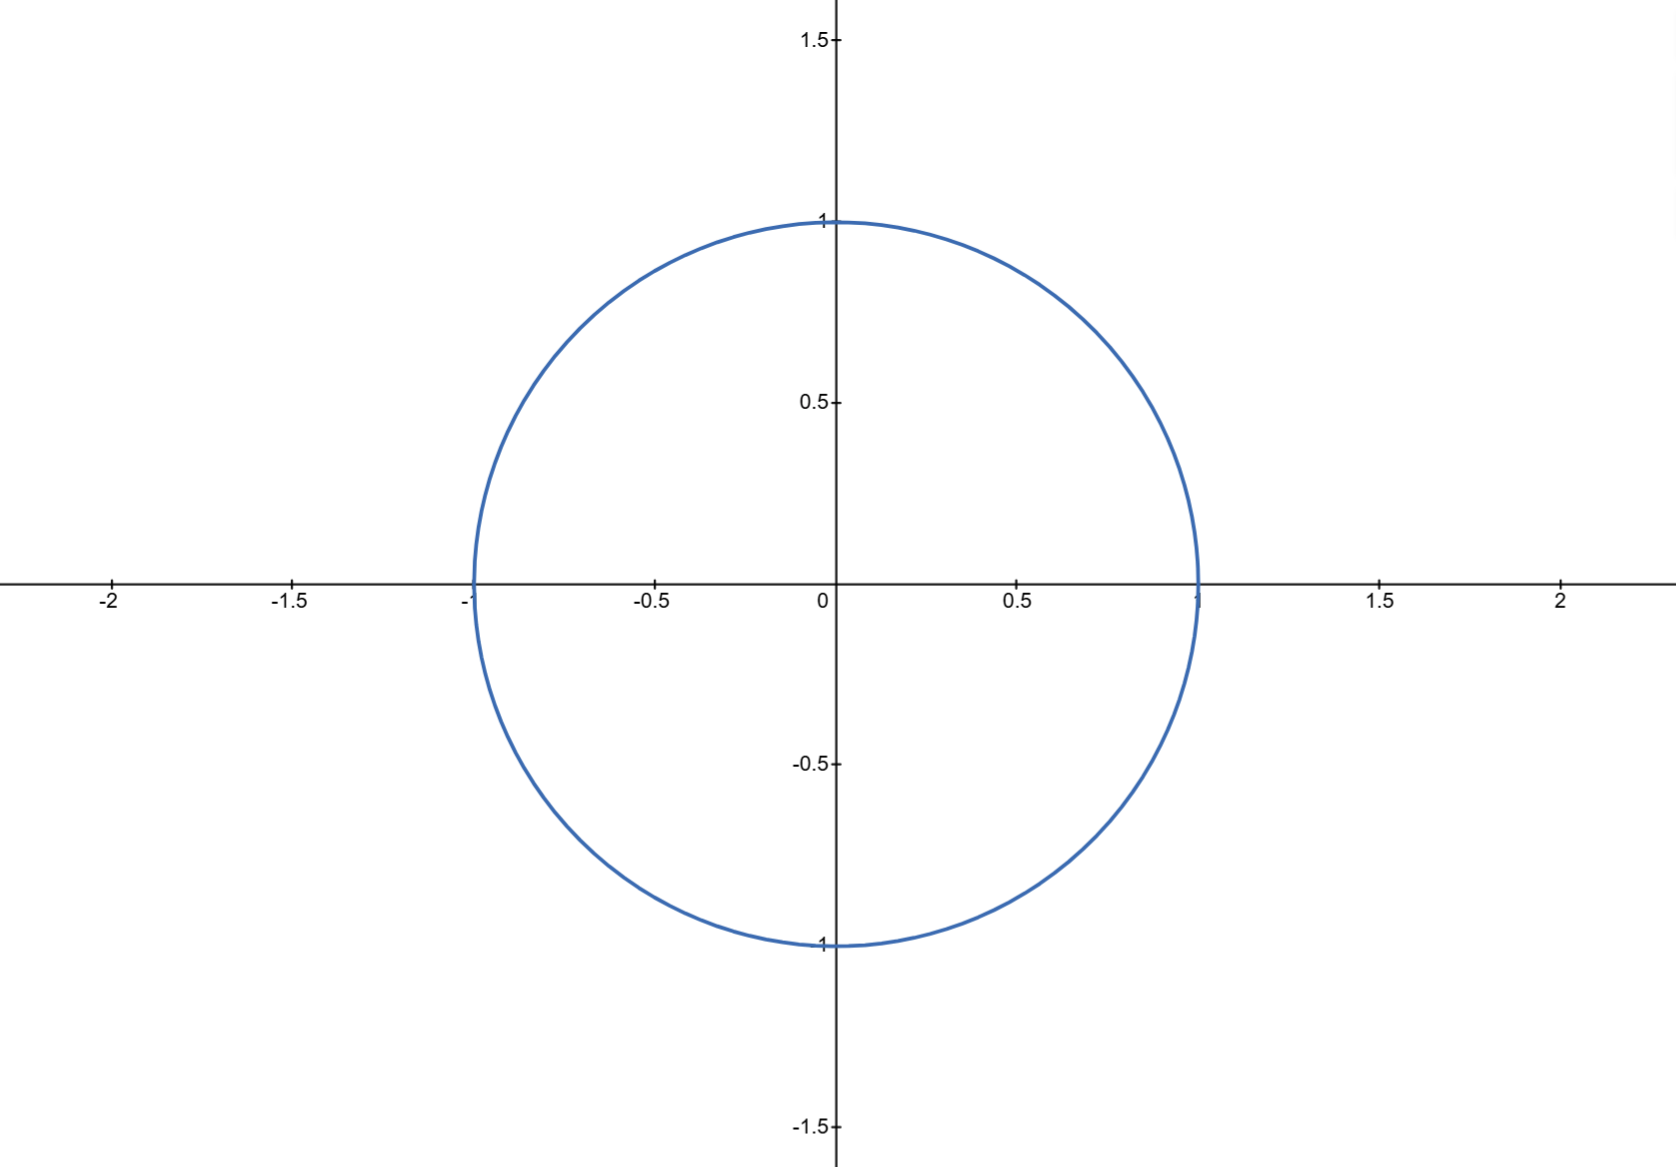
\includegraphics[width=0.6\textwidth]{img/unitCircle.png}
        \end{figure}
\end{columns}
\end{frame}

\begin{frame}{Ejercicio: Un cuadrado detrás de un circulo}
\begin{columns}
\column[t]{0.5\textwidth}
     \begin{itemize}
         \item Abstraer el código en funciones
         \item Tener una función que cambia las coordenadas
         \item Tener una función para el fondo
         \item Puedes utilizar la guía de colores
     \end{itemize}
\column[t]{0.5\textwidth}
        \begin{figure}[htb]
            \centering
            
\includegraphics[width=0.6\textwidth]{img/Ejer2}
            \caption{\url{https://github.com/nemediano}}
        \end{figure}
\end{columns}
\end{frame}

\begin{frame}{Transformaciones Afines}
Hay una definición formal de \href{https://en.wikipedia.org/wiki/Affine_transformation}{transformación afín}. Pero para nuestros propósitos, podremos decir que: una transformación afín $A: \mathbb{R}^n \rightarrow \mathbb{R}^n$ es una transformación lineal seguida de una traslación.

\begin{block}{}
    Si $\mathbf{x} \in \mathbb{R}^n$, $M$ es una matriz de $n \times n$ y $\mathbf{d} \in \mathbb{R}^n$ un vector.
    Entonces $A(\mathbf{x}) = M \mathbf{x} + \mathbf{d}$ es una transformación afín.
\end{block}
\begin{itemize}
    \item Todas las transformaciones lineales son transformaciones afines (con $\mathbf{d} = \mathbf{0}$)
    \item Todas las traslaciones son transformaciones afines (con $M = I$).
\end{itemize}
\end{frame}


\begin{frame}{Coordenadas homogéneas}

\begin{itemize}
    \item Todas las transformaciones lineales pueden llevarse a cabo multiplicando matrices.
    \item Pero las traslaciones no se pueden llevar a cabo multiplicando matrices
    \item Para solucionar ese problemas usamos las \href{https://en.wikipedia.org/wiki/Homogeneous_coordinates}{coordenadas homogéneas}
\end{itemize}
Vamos a adoptar la convención de que tanto puntos, como vectores son representados en columna.
\begin{block}{}
    Las coordenadas homogéneas de un punto $\mathbf{x} \in \mathbb{R}^n$, son una tupla de $n+1$ componentes, formada por los $n$ componentes de $\mathbf{x}$, seguidos por el escalar 1.
\end{block}
Ésta \emph{no es} la definición general, pero hará las explicaciones mas sencillas.
\begin{itemize}
    \item Las coordenadas homogéneas representan al punto $\mathbf{x} \in \mathbb{R}^n$ con un punto $\mathbf{x}_{h} \in \mathbb{R}^{n+1}$.
    \item Pero permiten \emph{expresar las transformaciones afines como una multiplicación de matrices}.
\end{itemize}

\end{frame}

\begin{frame}{Traslación}
\begin{columns}
\column[t]{0.5\textwidth}
\begin{itemize}
    \item Traslada una curva en el espacio
    \item Tiene parámetro el vector de traslación $\mathbf{t}$
    \item Se puede expresar con la siguiente matriz:
\end{itemize}
$$
\begin{pmatrix}
1 & 0 & t_x\\
0 & 1 & t_y\\
0 & 0 & 1
\end{pmatrix}
\begin{bmatrix}
x \\
y \\
1 \\
\end{bmatrix}
=
\begin{bmatrix}
x + t_x \\
y + t_y \\
1 \\
\end{bmatrix}
$$
\begin{itemize}
    \item Si $\mathbf{t} = \mathbf{0}$, hay una operación nula
    \item La operación inversa es trasladar por $-\mathbf{t}$
    \item La figura muestra una traslación por $\mathbf{t} = (2, 1)^t$
\end{itemize}
\column[t]{0.5\textwidth}
\begin{figure}[htp]
 \centering
 \begin{subfigure}[b]{0.4\textwidth}
   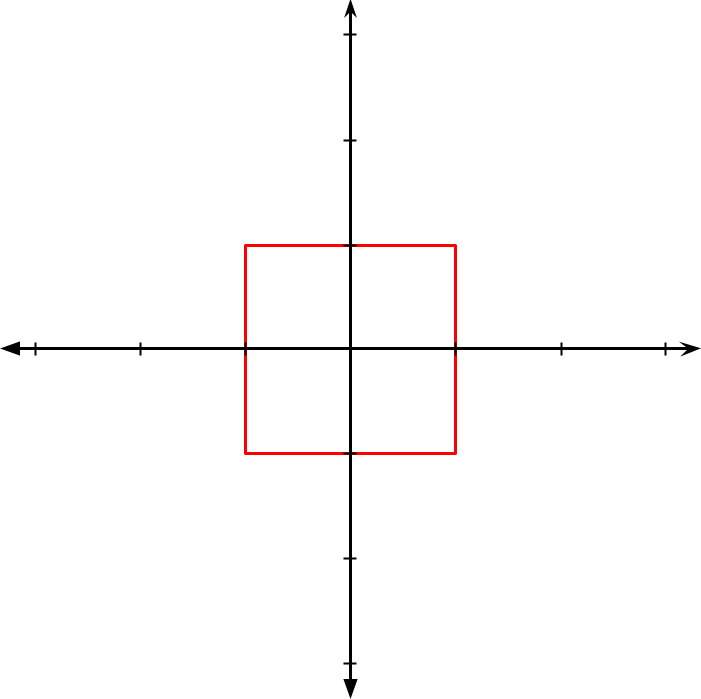
\includegraphics[width=\textwidth]{img/Square}
 \end{subfigure}
\\
\vspace{0.15cm}
 \begin{subfigure}[b]{0.4\textwidth}
   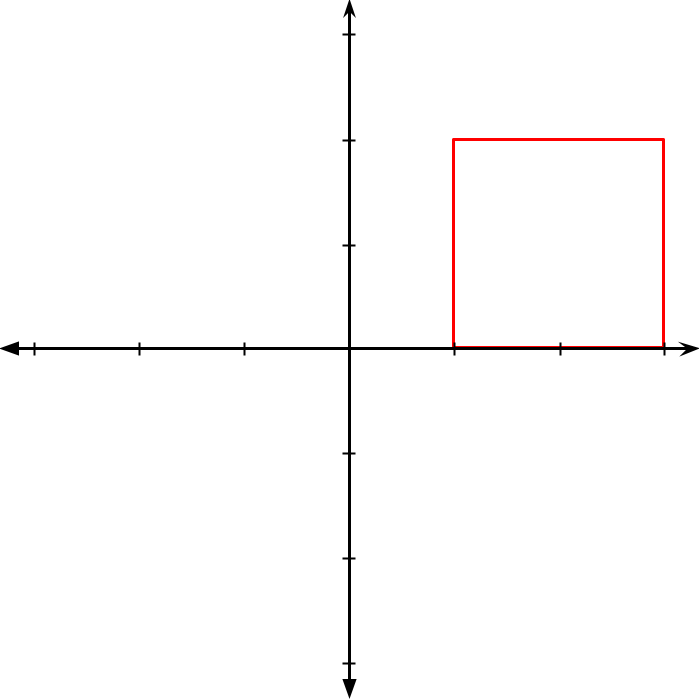
\includegraphics[width=\textwidth]{img/Translated}
 \end{subfigure}
\end{figure}
\end{columns}
\end{frame}

\begin{frame}{Rotación}
\begin{columns}
\column[t]{0.5\textwidth}
\begin{itemize}
    \item Rota una curva \emph{alrededor del origen}
    \item Tiene parámetro el angulo de rotación $\theta$
    \item Se puede expresar con la siguiente matriz:
\end{itemize}
$$
\begin{pmatrix}
\cos \theta & -\sin \theta & 0 \\
\sin \theta & \cos \theta & 0 \\
0 & 0 & 1
\end{pmatrix}
\begin{bmatrix}
x \\
y \\
1 \\
\end{bmatrix}
=
\begin{bmatrix}
x \cos \theta - y \sin \theta \\
x \sin \theta + y \cos \theta  \\
1 \\
\end{bmatrix}
$$
\begin{itemize}
    \item Si $\theta = 0$, hay una operación nula
    \item La operación inversa es rotar por $-\theta$
    \item La figura muestra una rotación de $\theta = \frac{\pi}{4}$
\end{itemize}
\column[t]{0.5\textwidth}
\begin{figure}[htp]
 \centering
 \begin{subfigure}[b]{0.4\textwidth}
   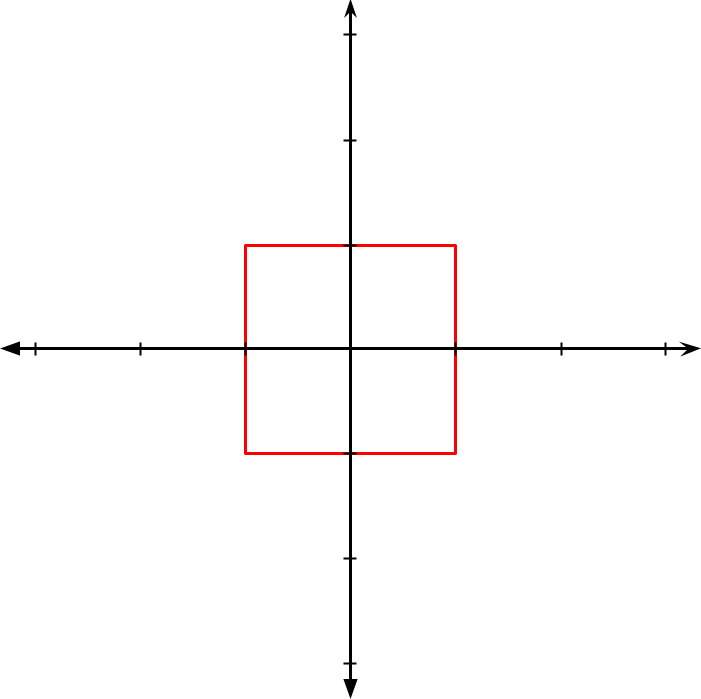
\includegraphics[width=\textwidth]{img/Square}
 \end{subfigure}
\\
\vspace{0.15cm}
 \begin{subfigure}[b]{0.4\textwidth}
   
\includegraphics[width=\textwidth]{img/Rotated}
 \end{subfigure}
\end{figure}
\end{columns}
\end{frame}

\begin{frame}{Escalamiento}
\begin{columns}
\column[t]{0.5\textwidth}
\begin{itemize}
    \item Escala una curva \emph{con respecto al origen}
    \item Tiene parámetro el factor de escala $\mathbf{s}$
    \item Se puede expresar con la siguiente matriz:
\end{itemize}
$$
\begin{pmatrix}
s_x & 0 & 0 \\
0 & s_y & 0 \\
0 & 0 & 1
\end{pmatrix}
\begin{bmatrix}
x \\
y \\
1 \\
\end{bmatrix}
=
\begin{bmatrix}
s_x \cdot x  \\
s_y \cdot y  \\
1 \\
\end{bmatrix}
$$
\begin{itemize}
    \item Si $\mathbf{s} = ( 1 , 1 )^t$, hay una operación nula
    \item La operación inversa es escalar por $\mathbf{s} = (\frac{1}{s_x} , \frac{1}{s_y} )^t$
    \item La figura muestra un escalamiento por $\mathbf{s} = ( \frac{1}{2} , 2 )^t$
\end{itemize}
\column[t]{0.5\textwidth}
\begin{figure}[htp]
 \centering
 \begin{subfigure}[b]{0.4\textwidth}
   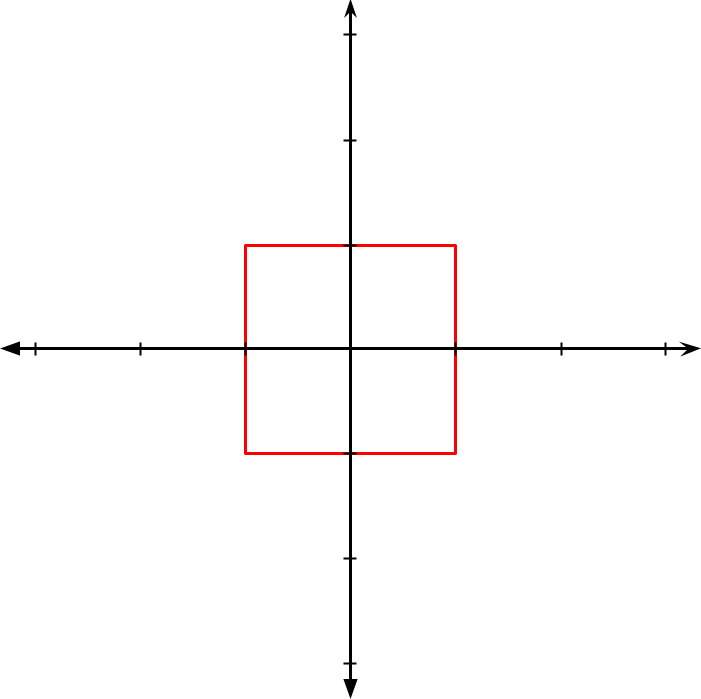
\includegraphics[width=\textwidth]{img/Square}
 \end{subfigure}
\\
\vspace{0.15cm}
 \begin{subfigure}[b]{0.4\textwidth}
   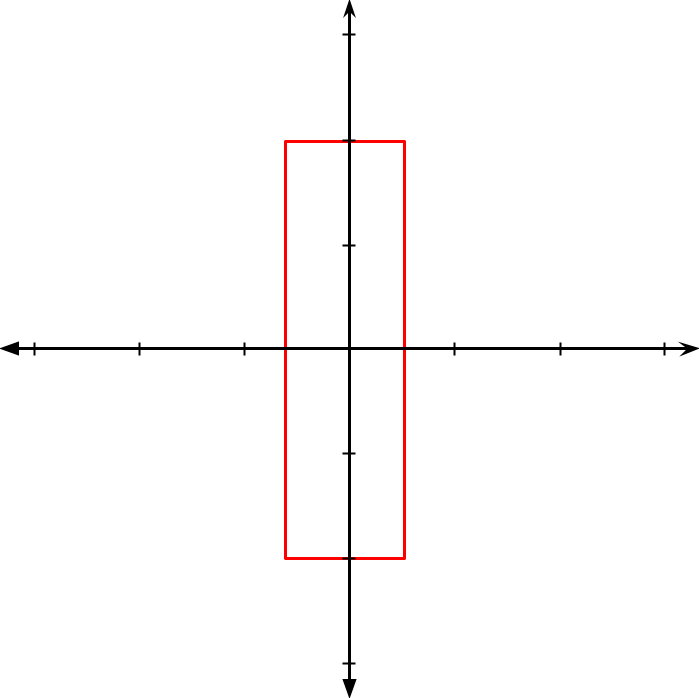
\includegraphics[width=\textwidth]{img/Scalated}
 \end{subfigure}
\end{figure}
\end{columns}
\end{frame}

\begin{frame}{Composición de transformaciones afines}
Las transformaciones afines, se pueden aplicar una después de otra. 
\begin{itemize}
    \item Esto se llama \alert{composición de transformaciones}
    \item Y es particularmente útil que se haga con matrices
    \item La multiplicación de matrices es asociativa 
    $$T_1 T_2 T_3 \mathbf{x} = T_1 (T_2 (T_3 \mathbf{x})) = (T_1 T_2 T_3) \mathbf{x}$$
    \item La multiplicación de matrices no es conmutativa: 
    $$T_1 T_2 \mathbf{x} \neq T_2 T_1 \mathbf{x}$$
\end{itemize}
\end{frame}

\begin{frame}{Ejemplo}
Si $R$ fuera una rotación de $\frac{5\pi}{4}$ y $S$ escalameinto por $(\frac{1}{2}, 2)^t$
\begin{figure}[htp]
 \centering
 \begin{subfigure}[b]{0.25\textwidth}
   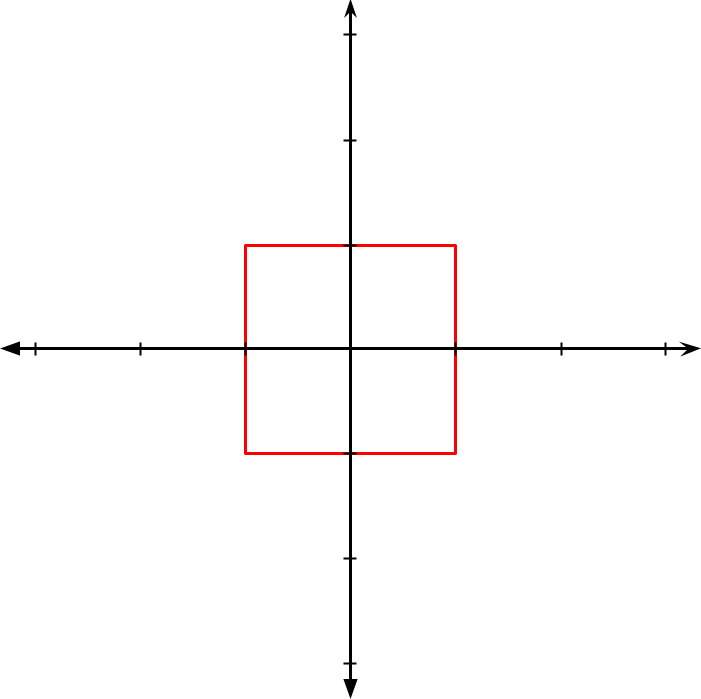
\includegraphics[width=\textwidth]{img/Square}
   \caption{Figura original}
 \end{subfigure}
 ~
 \begin{subfigure}[b]{0.25\textwidth}
   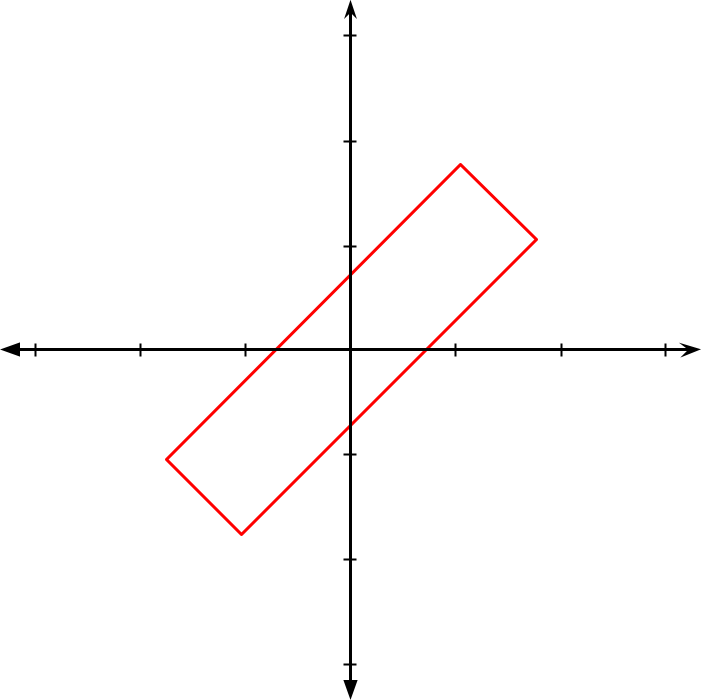
\includegraphics[width=\textwidth]{img/ScaleRoate}
   \caption{$R S \mathbf{x} = ( R ( S \mathbf{x}))$}
 \end{subfigure}
 ~
 \begin{subfigure}[b]{0.25\textwidth}
   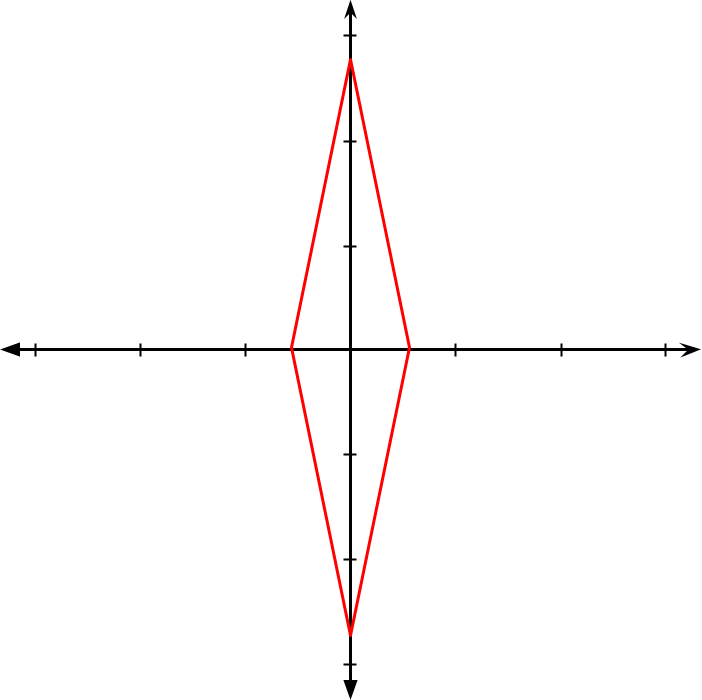
\includegraphics[width=\textwidth]{img/RoateScale}
   \caption{$S R \mathbf{x} = (S (R \mathbf{x}))$}
 \end{subfigure}
\end{figure}
\end{frame}

\begin{frame}{Transformaciones afines en Shadertoy}
\begin{itemize}
    \item La explicación anterior es como se hacen las gráficas tradicionalmente.
    \item Es decir, transformamos la geométrica para acomodarla en el espacio.
\end{itemize}
\begin{alertblock}{En Shadertoy en 2D hacemos lo contrario}
    \begin{itemize}
        \item En shadertoy en 2D, trasformamos las coordenadas del fragment hacia la figura.
        \item Esto es equivalente a decir que transformamos el espacio hacia la figura.
        \item Por lo tanto, para situar figuras en 2D usamos la matriz inversa de la matriz de trasformación.
    \end{itemize}
\end{alertblock}
\end{frame}

\begin{frame}[fragile]{Ejemplo en Shadertoy 2D}
\begin{listing}
\begin{minted}{glsl}
mat3 M = translate(vec2(0.75, 0.0)) * scale(vec2(0.25));

float disCircle = sdfCircle(inverse(M) * coord);

color = mix(Red, color, step(0.0, disCircle));
\end{minted}
\end{listing}
\begin{itemize}
    \item En este ejemplo se escala y luego se traslada una figura (circulo)
    \item Nótese la inversión de la matriz, antes de evaluar las sdf.
    \item Y el uso de la función \mintinline{glsl}{step} dentro de la función \mintinline{glsl}{mix}, para cambiar el color del fragment si estaba dentro de la figura.
\end{itemize}
\end{frame}

\begin{frame}{Ejercicio: Figuras animadas}
\begin{columns}
\column[t]{0.5\textwidth}
     \begin{itemize}
         \item Usar transformaciones compuestas para crear una escena
         \item Puedes utilizar la \href{https://iquilezles.org/articles/distfunctions2d/}{esta lista} para ver mas figuras
         \item Puedes comenzar con el código del ejercicio anterior 
     \end{itemize}
\column[t]{0.5\textwidth}
        \begin{figure}[htb]
            \centering
            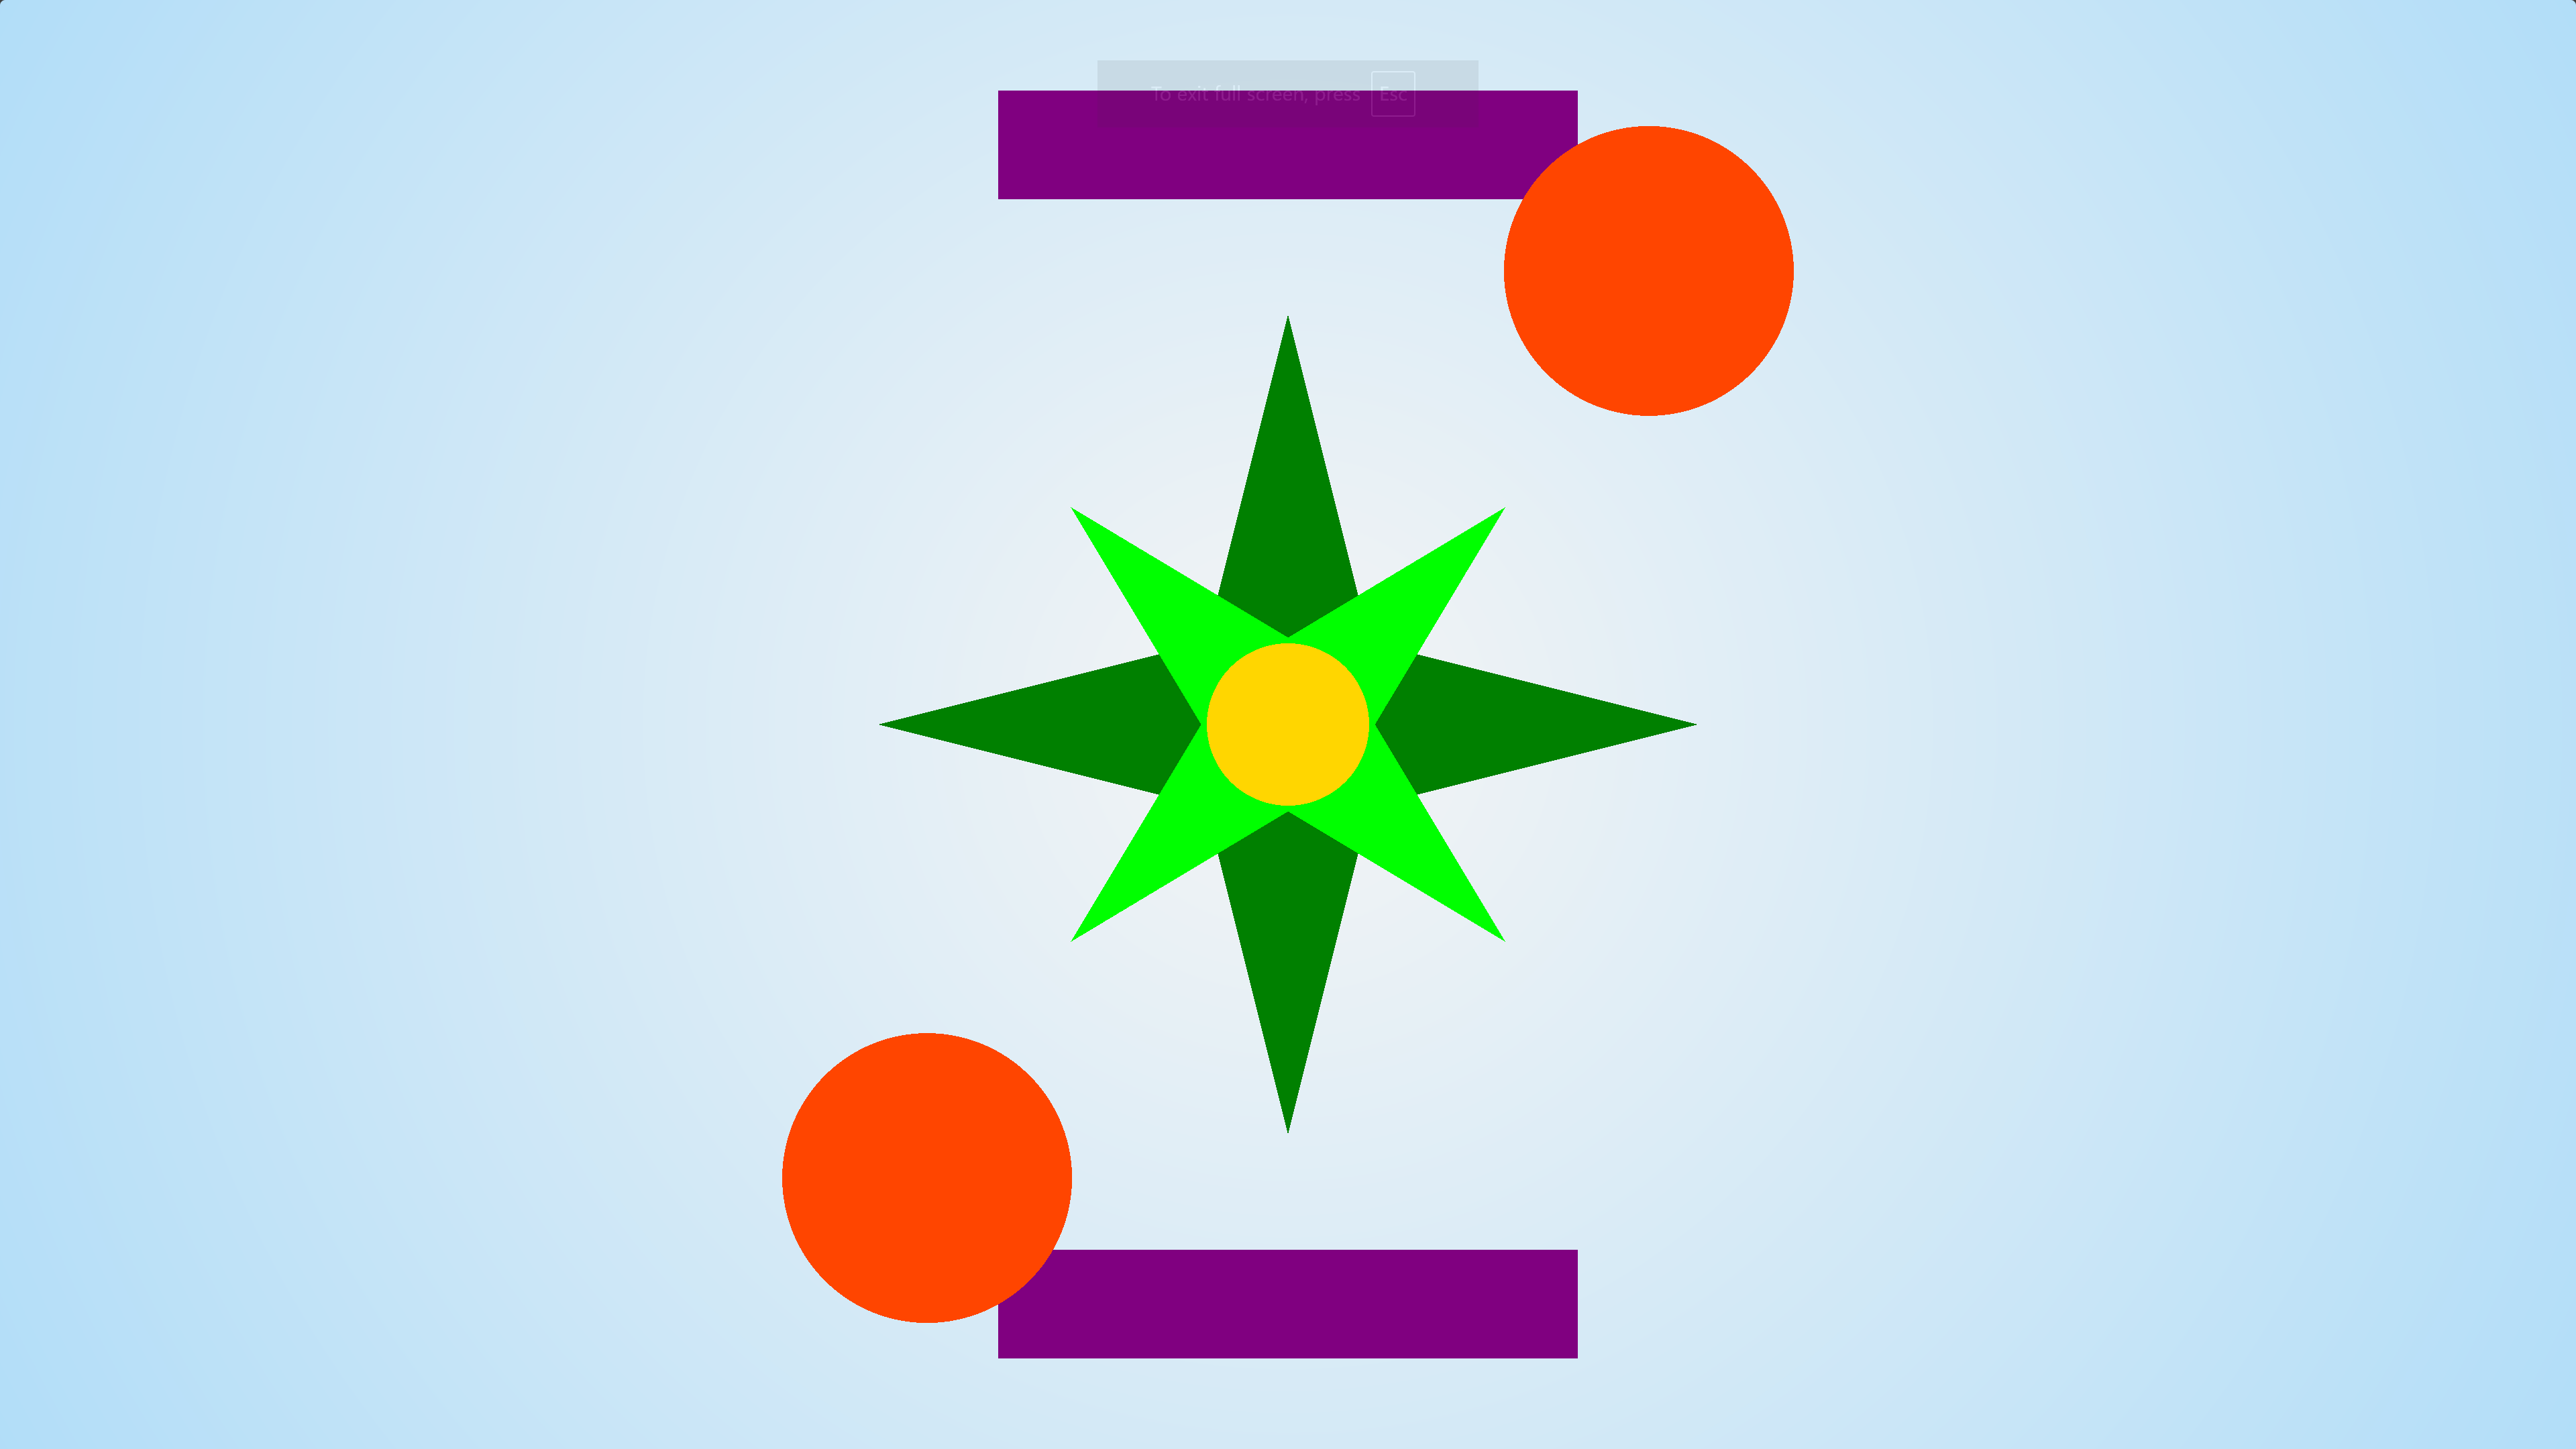
\includegraphics[width=0.6\textwidth]{img/Ejer3}
            \caption{\url{https://github.com/nemediano}}
        \end{figure}
\end{columns}
\end{frame}

\section{Ray marching}
\begin{frame}{Algoritmos basados en rayos}
En realidad esta es un familia de algoritmos, los mas importantes son:

\begin{itemize}
    \item \href{https://en.wikipedia.org/wiki/Ray_casting}{Ray Casting:} El primero en ser desarrollado. Consiste en lanzar un rayo por cada pixel del viewport. Para ver donde interfecta la escena.
    \item \href{https://en.wikipedia.org/wiki/Ray_tracing_(graphics)}{Ray Tracing:} Una generalización donde cada vez que se intersecta la escena, se calcula el angulo de reflexión y se continua siguiendo el rayo, hasta cumplir algún criterio de paro.
    \item \href{https://en.wikipedia.org/wiki/Ray_marching}{Ray Marching:} Una forma de usar la sdf, para acelerar el camino de los rayos de manera recursiva. Este es el mas usado en ShaderToy
    \item \href{https://en.wikipedia.org/wiki/Path_tracing}{Path Tracing:} En vez de lanzar un rayo, se lanzan varios rayos a ángulos muy similares usando el método de Monte Carlo.
\end{itemize}

\end{frame}

\begin{frame}{El rayo}
\begin{block}{Rayo}
Un rayo es el semisegemento de linea $\mathbf{r}(s) = \mathbf{o} + s  \mathbf{d}$, donde $s \in \mathbb{R}^{+}$ es un escalar positivo, $\mathbf{o}$ es un punto en $\mathbb{R}^3$ y $|\mathbf{d}| = 1$ un vector unitario en $\mathbb{R}^3$. 

\end{block}

\begin{columns}
\column[t]{0.5\textwidth}
\begin{itemize}
    \item $\mathbf{o}$ es el origen del rayo.
    \item $\mathbf{d}$ es la dirección del rayo.
    \item $s$ es el parámetro.
\end{itemize}    
\column[t]{0.5\textwidth}
\begin{figure}[htp]
    \centering
    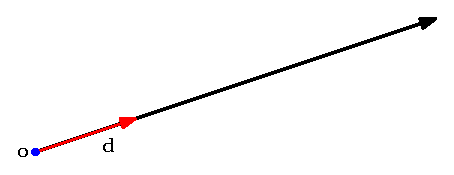
\includegraphics[width=0.6\textwidth]{img/ray.eps}    
\end{figure}
\end{columns}
\end{frame}

\begin{frame}{Ray Marching}
Es una técnica para hacer un avance adaptativo de lo rayos.
\begin{enumerate}
    \item En el punto actual del rayo calcula la distancia $d$ del punto con respecto a la escena.
    La \emph{distancia} de la escena, es la mínima de todas las sdfs a las figuras en la escena.
    \item Si $d$ es menor que un cierto $\epsilon$, termina y reporta que hay una colisión con la escena.
    \item Si $d$ es mayor que un cierto valor frontera termina y di que no hay colisión.
    \item Avanza el rayo en $d$ unidades, y repite desde 1.
\end{enumerate}
Esta técnica solo se puede usar si\ldots
\begin{itemize}
    \item Definimos la escena por medio de sdfs.
    \item El rayo tiene un vector de dirección unitario.
    \item Las sdf están bien definidas:
    \begin{itemize}
        \item Continuas.
        \item La distancia esta en la misma dimensión que la escena.
    \end{itemize}    
\end{itemize}

\end{frame}

\begin{frame}{Ray Marching: una imagen}

\begin{itemize}
    \item En la practica se pone un numero máximo de pasos como criterio extra de paro.
\end{itemize}    

\begin{figure}[htp]
    \centering
    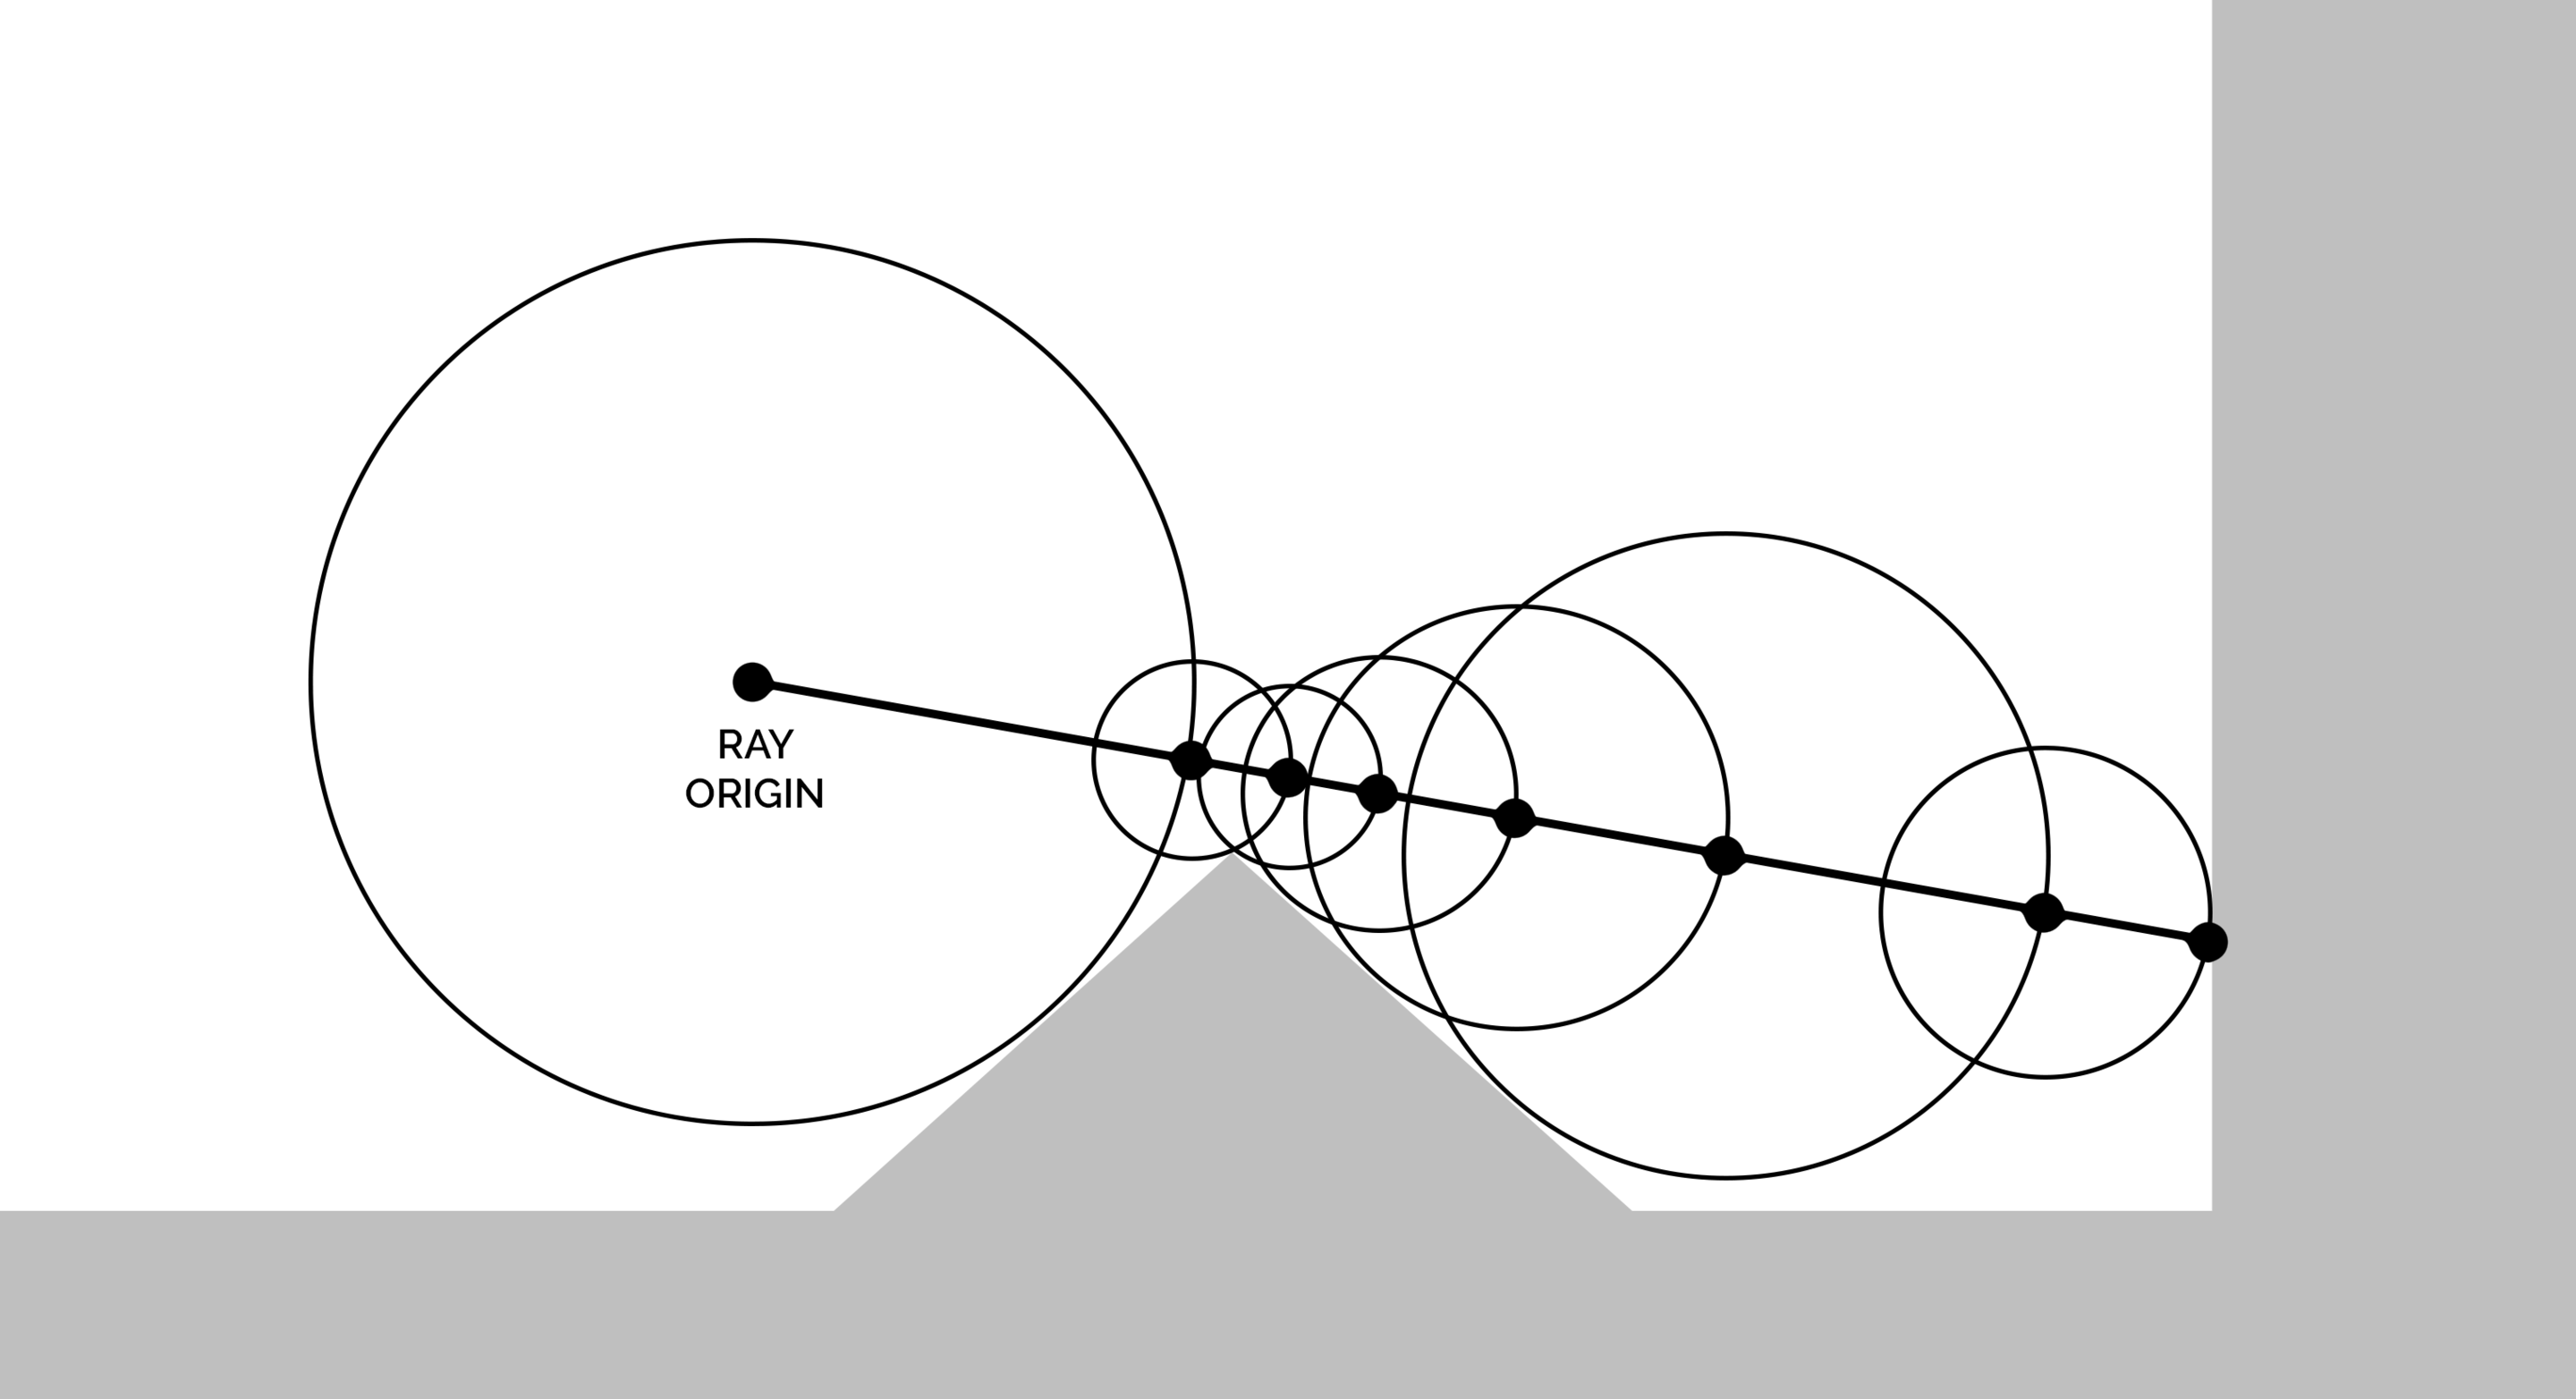
\includegraphics[width=0.6\textwidth]{img/rayMarch}    
\end{figure}

Hay un \href{https://www.shadertoy.com/view/4dSfRc}{ejemplo} para visualizar la técnica en ShaderToy mismo.

\end{frame}

\begin{frame}[fragile]{Ray Marching: en código}
\begin{listing}
\begin{minted}{glsl}
float rayMarch(Ray ray, float start, float end) {
  float depth = start;

  for (int i = 0; i < MAX_MARCHING_STEPS; i++) {
    vec3 position = ray.origin + depth * ray.direction;
    float d = sdScene(position);
    depth += d;
    if (d < PRECISION || depth > end) break;
  }

  return depth;
}
\end{minted}
\end{listing}

\end{frame}

\begin{frame}{Visualizar en 3D}
\begin{itemize}
    \item Para no ver todo de un color plano en 3D, necesitamos hacer shading.
    \item Para hacer shading, necesitamos (entre otras cosas), la normal $\mathbf{n}$ a la superficie en el punto de contacto.
    \item Podemos utilizar la misma sdf, para calcular el gradiente $\nabla$ de la figura. El gradiente es una buena aproximación a la normal: $\nabla \approx \mathbf{n}$.
\end{itemize}
$$\nabla (f(\mathbf{x})) = \begin{pmatrix}
f(x + \epsilon, y, z) - f(x - \epsilon, y, z)\\
f(x, y + \epsilon, z) - f(x, y - \epsilon, z)\\
f(x, y, z + \epsilon) - f(x, y, z - \epsilon)
\end{pmatrix}$$
Donde $f(\mathbf{x})$ es una sdf y $\epsilon$ un numero positivo muy pequeño.
\begin{itemize}
    \item Finalmente, si definimos una fuente de luz, con una posición $\mathbf{l}$ en la escena.
    \item Una forma muy sencilla de shading puede ser: $c = \max(\mathbf{k}_d (\mathbf{l} \cdot \mathbf{n}), \mathbf{0})$.
    \item Donde $\mathbf{c}$ es el color resultante y $\mathbf{k}_s$ es el color predominante de la superficie.
\end{itemize}
\end{frame}

\begin{frame}{Ejercicio: Esfera usando Ray Marching}
\url{https://github.com/nemediano/tallerShadertoy/tree/main/codigo/Ejercicio4}
\begin{columns}
\column[t]{0.5\textwidth}
     \begin{itemize}
         \item De momento, usa solo una esfera en la escena.
         \item Trata de definir tu cámara, la esfera y una fuente de luz, en lugares sencillos respecto al origen.
         \item De momento usa la reflexión difusa, para que puedas visualizar al esfera.
         \item Puedes usar el código de comienzo de la escena para empezar.
     \end{itemize}
\column[t]{0.5\textwidth}
        \begin{figure}[htb]
            \centering
            
\includegraphics[width=0.6\textwidth]{img/Ejer/Ejer4}
        \end{figure}
\end{columns}
\end{frame}

\begin{frame}{¿Qué mas podemos añadir?}

En lo que resta del taller vamos a añadir algunas cosas al ejemplo de Raymarching:

\begin{enumerate}
    \item Como manejar una escena con varios objetos.
    \item Como hacer un modelo de cámara mas robusto.
    \item El modelo de iluminación de Blin-Phong.
    \item \href{https://en.wikipedia.org/wiki/Constructive_solid_geometry}{Constructive solid geometry} gracias a las sdf.
\end{enumerate}

\end{frame}

\subsection{Escena con mas de un objeto}
\begin{frame}[fragile]{Generalizar la escena para varios objetos}
Actualmente, la escena esta definida por una sola sdf.
Para hacer el código mas general hay varios métodos.
Aquí solo voy a explicar uno de ellos.

\begin{itemize}
    \item Definir una estructura mas general que represente un punto en la escena.
    \item De momento contiene un escalar que representa la distancia del punto sobre el rayo.
    \item Para demostrar la utilidad vamos a incluir un campo extra (el color).
\end{itemize}

\begin{listing}
\begin{minted}{glsl}
struct ScenePoint {
  float dist;
  vec3 color;
};
\end{minted}
\end{listing}

\end{frame}

\begin{frame}[fragile]{Mas detalles\ldots}
\begin{itemize}
    \item La función \mintinline{glsl}{sdScene} debería regresar ahora un \mintinline{glsl}{ScenePoint}.
    \item Por supuesto, esto requiere cambiar \mintinline{glsl}{calcNormal}
    \item Y por ultimo, también cambiar \mintinline{glsl}{RayMarch} para regresar un \mintinline{glsl}{ScenePoint}. 
\end{itemize}

\begin{block}{¿Qué necesitamos saber de un punto en la escena?}
    \begin{itemize}
        \item Antes, lo único que necesitábamos para identificar un punto en la escena era la distancia a la que debíamos marchar el rayo.
        
        \item Solo le estamos poniendo mas información a ese punto.
    \end{itemize}
\end{block}

\begin{block}{¿Como se manejan varios objetos en la escena?}
    \begin{itemize}
        \item La función \mintinline{glsl}{sdScene} debe de regresar la \alert{distancia mínima} de la distancias a todos los objetos de la escena. 
        
        \item La escena es un objeto formado por todos los objetos que contiene. Por lo tanto, la \say{sdf de la escena} esta definida como la mínima de todas las distancias.
    \end{itemize}
\end{block}
\end{frame}

\begin{frame}[fragile]{Agregando el piso de la escena}
Podemos definir fácilmente la sdf de un semiespcacio ortogonal al eje $y$.
\begin{listing}
\begin{minted}{glsl}
float sdFloor(vec3 position, float floorHeight) {
    return position.y - floorHeight;
}
\end{minted}
\end{listing}
Y podemos definir un color en términos de una posición en el plano $xy$, por ejemplo para crear un patrón de \say{tablero de ajedrez}.
\begin{listing}
\begin{minted}{glsl}
vec3 getCheckboardPattern(vec2 coords, vec3 colorEven, vec3 colorOdd) {
    float alpha = mod(floor(coords.x) + floor(coords.y), 2.0);
    return mix(colorEven, colorOdd, alpha);
}
\end{minted}
\end{listing}

\end{frame}

\begin{frame}[fragile]{Ejemplo de sdf con varios objetos}
\begin{listing}
\begin{minted}{glsl}
ScenePoint sdScene(vec3 position) {
  ScenePoint closestShape;
  // Closest shape is the first shape (the floor)
  closestShape.dist = sdFloor(position, -1.0);
  closestShape.color = getCheckboardPattern(position.xz, vec3(1.0), vec3(1.4));
  // Now test the second shape (a box)
  float testDistance = sdBox(position, vec3(1.5, 0.0, 0.0), vec3(1.0));
  // If this shape is closer, update closest shape
  if (testDistance < closestShape.dist) {
    closestShape.dist = testDistance;
    closestShape.color = DarkSeaGreen;
  }

  return closestShape;
}
\end{minted}
\end{listing}
\end{frame}

\subsection{Un modelo de cámara}

\begin{frame}{Un modelo de cámara típico}
En CG, la cámara esta definida con dos matrices:
\begin{enumerate}
  \item La de \alert{vista}: Que contiene la \href{https://en.wikipedia.org/wiki/Pose_(computer_vision)}{pose} de la cámara.
  \item La de \alert{proyección}: Que define el volumen de visión de la cámara.
\end{enumerate}
\begin{itemize}
   \item Una \say{pose} es una posición, en el espacio junto con una orientación (dirección).
   \begin{itemize}
     \item Típicamente, se usan un punto en $\mathbb{R}^3$ y un \href{https://en.wikipedia.org/wiki/Quaternion}{cuaternión}. Por lo que tiene 7 grados de libertad.
     \item Piensa en ella como posicionar tu cámara usando un \href{https://en.wikipedia.org/wiki/Tripod_(photography)}{tripié}
   \end{itemize}
   \item Cuando decimos proyección, generalmente queremos decir \href{https://en.wikipedia.org/wiki/3D_projection\#Perspective_projection}{proyección en perspectiva}.
   \begin{itemize}
     \item Se define con una proporción del plano (\emph{aspect ratio}) y dos distancias: la cercana y la lejana.
     \item Piensa en ella como configurar tu cámara: escoger el lente adecuado, ajustar el zoom, etc.
   \end{itemize}
\end{itemize}
\begin{block}{}
 En nuestro caso la proyección esta implícita en el algoritmo de Ray Marching.
 \begin{itemize}
   \item Solo nos hace falta construir la matriz de vista.
 \end{itemize}
\end{block}
\end{frame}

\begin{frame}[fragile]{La pose de la cámara}
Hay varias maneras de definir una pose para nuestra cámara.
\begin{itemize}
    \item No necesitamos la matriz de vista completa
    \item Una posibilidad es usar el modelo \say{Look at} que se define con dos puntos y un vector:
    \begin{itemize}
        \item El centro de visión (posición de la cámara)
        \item El objetivo (el punto en la escena que quieres enfocar)
        \item El vector arriba (generalmente el eje $y$).
    \end{itemize}
    \item Lo vamos a simplificar a un vector arriba fijo, por lo que solo necesitaremos los dos puntos. Puedes consultar la teoría \href{https://learnopengl.com/Getting-started/Camera}{aquí}.
\end{itemize}
\begin{listing}
\begin{minted}{glsl}
mat3 camRotation(Camera cam) {
    vec3 camDir = normalize(cam.target - cam.position);
    vec3 camRight = normalize(cross(vec3(0, 1, 0), camDir));
    vec3 camUp = normalize(cross(camDir, camRight));

    return mat3(-camRight, camUp, -camDir);
}
\end{minted}
\end{listing}
\end{frame}

\begin{frame}[fragile]{La pose de la cámara}
Para nuestro caso, rotar la cámara significa rotar la dirección de los rayos:
\begin{listing}
\begin{minted}{glsl}
Camera cam;
cam.position = vec3(0.0, 1.0, 2.0);
cam.target = vec3(0.0);

Ray ray;
ray.origin = cam.position;
ray.direction = camRotation(cam) * normalize(vec3(coord.xy, -1.0));
\end{minted}
\end{listing}
\end{frame}

\subsection{El modelo de iluminación de Blin-Phong}

\begin{frame}{El modelo de iluminación de Blin-Phong}
\begin{columns}
\column[t]{0.5\textwidth}
\begin{itemize}
 \item En 1975 \href{https://en.wikipedia.org/wiki/Phong_reflection_model}{Bui Tuong Phong} desarolló un modelo de iluminación.
 \item La reflexion de la luz se divide en tres coponentes: ambiente, difusso y especular.
 \item En 1977 \href{https://en.wikipedia.org/wiki/Blinn-Phong_reflection_model}{Jim Blinn}, modificó el calculo del componente especular para hacerlo mas estable y mas eficiente.
 \item Es el modelo de \say{shading sencillo}, mas usado.
\end{itemize}
\column[t]{0.5\textwidth}
\begin{figure}[htp]
 \centering
 \begin{subfigure}[b]{0.42\textwidth}
   
\includegraphics[width=\textwidth]{img/ambiente}
   \caption{Ambiente}
 \end{subfigure}
~
 \begin{subfigure}[b]{0.42\textwidth}
   
\includegraphics[width=\textwidth]{img/difuso}
   \caption{Difuso}
 \end{subfigure}
\\
 \begin{subfigure}[b]{0.42\textwidth}
   
\includegraphics[width=\textwidth]{img/especular}
   \caption{Especular}
 \end{subfigure}
~
 \begin{subfigure}[b]{0.42\textwidth}
   
\includegraphics[width=\textwidth]{img/completo}
   \caption{Completo}
 \end{subfigure}
\end{figure} 
\end{columns}
\end{frame}

\begin{frame}{¿Cómo se calcula la reflexión?}
La reflexión de la luz (color) de un punto en la superficie se calcula como:
 $$\mathbf{L}_a \mathbf{K}_a + \mathbf{L}_d \mathbf{K}_d (\mathbf{n} \cdot \mathbf{l}) + \mathbf{L}_s \mathbf{K}_s (\mathbf{v} \cdot \mathbf{h})^{\alpha}$$
 En donde:
 \begin{itemize}
  \item $\mathbf{L}$ son los tres colores (ambiente, difuso y especular) de la luz 
  \item $\mathbf{K}$ son los tres colores (ambiente, difuso y especular) del material.
  \item $\alpha$ es la constante del brillo del material
  \item $\mathbf{n}$ la normal a la superficie en el punto
  \item $\mathbf{l}$ un vector unitario que apunta a la fuente de luz desde el punto
  \item $\mathbf{v}$ un vector unitario que apunta a la camara desde el punto
  \item $\mathbf{h} = \frac{\mathbf{l} + \mathbf{v}}{|\mathbf{l} + \mathbf{v}|}$ un vector unitario, llamado \say{halfway vector}.
 \end{itemize}
\end{frame}


\begin{frame}{Detalles de implementación}
\begin{itemize}
  \item A cada objeto de la escena se le asiga un material en vez de un color
  \item En escenas simples, se aconseja definir la luz como blanco intenso; para evitar complicaciones.
   \item El material esta formado por tres colores ($\mathbf{K}_a, \mathbf{K}_d, \mathbf{K}_s$) y un escalar ($\alpha$)
   \item Usualmente restringimos $\alpha \in [ 0.5, 128 ]$, y cuando experimenatmos, la variamos logaritmicamente.
  \begin{itemize}
   \item Un $\alpha$ grande produce brillos pequeños y concentrados.
   \item Un $\alpha$ pequeño produce brillos grandes y débiles.
  \end{itemize}
  \item Dado que no se puede \say{restar luz}, los productos puntos $\mathbf{n} \cdot \mathbf{l}$ y $\mathbf{v} \cdot \mathbf{h}$ deben ser no negativos.
  \item Si hay mas de una luz en la escena:
  \begin{itemize}
   \item Se calcula el componente normal una vez.
   \item Y los componentes difuso y especular una vez por cada luz, acumulando (sumando) el resultado
  \end{itemize}
\end{itemize}
\end{frame}

\begin{frame}{Ejercicio: Mejorar el Ray Marching anterior}
\url{https://github.com/nemediano/tallerShadertoy/tree/main/codigo/Ejercicio5}
\begin{columns}
\column[t]{0.5\textwidth}
     \begin{itemize}
         \item Lógica para desplegar varios objetos en la escena, uno de ellos un piso.
         \item La cámara se define con el modelo LookAt. Idealmente una cámara que gire alrededor de la escena.
         \item Utilice el algoritmo de Blinn–Phong para hacer el shading
     \end{itemize}
\column[t]{0.5\textwidth}
        \begin{figure}[htb]
            \centering
            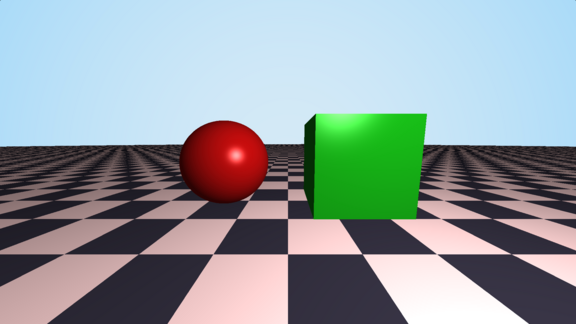
\includegraphics[width=0.6\textwidth]{img/Ejer/Ejer5}
        \end{figure}
\end{columns}
\end{frame}

\subsection{Modelado geométrico usando las sdf}

\begin{frame}{Transformaciones afines de 3D}
\begin{itemize}
    \item Las transformaciones afines se pueden generalizar a 3D.
    \item La traslación y el escalamiento se generalizan de manera trivial.
    \item La rotación en 3D, requiere de un parámetro extra: un \alert{vector} unitario que nos sirve de eje de rotación.
    \begin{itemize}
        \item La rotación sigue siendo con respecto al origen.
        \item Recuerda, que los vectores son libres en el espacio.
    \end{itemize}
    \item Aquí solo usaremos una función que nos devuelve la matriz de rotación a partir de un angulo y un vector.
    \item Puedes ver como se construye en el excelente libro: \href{https://mathweb.ucsd.edu/~sbuss/CourseWeb/Math155A_2019Winter/SecondEdDraft.pdf}{3D Computer Graphics: A mathematical approach with OpenGL}
    
\end{itemize}
\end{frame}

\begin{frame}[fragile]{Signed distance functions en 3D}
\begin{block}{¿Dónde puedo buscar mas sdf?}
    El mejor lugar para buscar una sdf es el \href{https://iquilezles.org/articles/distfunctions/}{sitio personal} de Inigo Quilez
\end{block}
Para aumentar el poder de expresividad, puedes pasar un parámetro extra que sea la transformación afín.
Para un cubo por ejemplo:
\begin{listing}
\begin{minted}{glsl}
float sdBox(vec3 position, vec3 boxCenter, vec3 boxSizes) {
  vec3 q = abs(position - boxCenter) - boxSizes;
  return length(max(q, 0.0)) + min(max(q.x, max(q.y, q.z)), 0.0);
}

float sdBox(vec3 position, mat4 T) {
  vec3 tPos = (inverse(T) * vec4(position, 1.0)).xyz;
  vec3 q = abs(tPos) - vec3(1.0);
  return length(max(q, 0.0)) + min(max(q.x, max(q.y, q.z)), 0.0);
}
\end{minted}
\end{listing}

\end{frame}

\begin{frame}{Deformando el espacio}

\begin{itemize}
    \item Escalar \alert{deforma el espacio} y eso afecta las funciones de distancia.
    \item El Ray Marching es mas tolerable a expandir el espacio que a contraer el espacio. Es decir, es \alert{posible} que escalar por números mayores que uno funcione.
    \item Algunas sdf pueden escalarse directamente desde la formula. La Figura muestra una caja (cubo) escalado en: $(\frac{1}{2}, 1, \frac{1}{2})$ por ambos métodos.
\end{itemize}

\begin{figure}[htp]
 \centering
 \begin{subfigure}[b]{0.22\textwidth}
   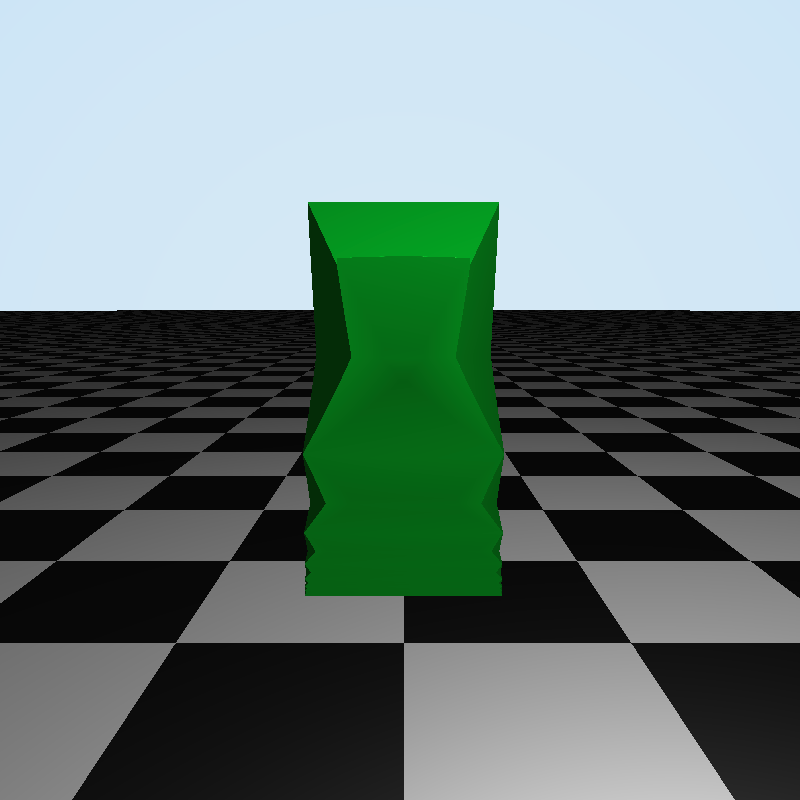
\includegraphics[width=\textwidth]{img/inestable}
   \caption{Matriz}
 \end{subfigure}
~
 \begin{subfigure}[b]{0.22\textwidth}
   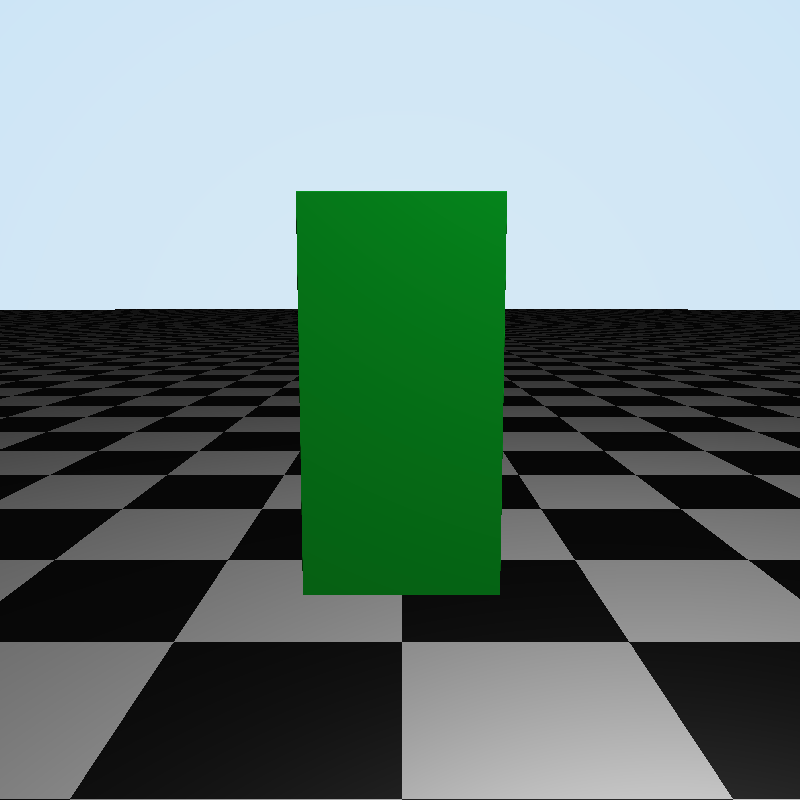
\includegraphics[width=\textwidth]{img/estable}
   \caption{Formula}
 \end{subfigure}
\end{figure} 

\end{frame}

\begin{frame}{Constructive Solid Geometry}

\begin{columns}
\column[t]{0.5\textwidth}
\begin{itemize}
    \item La \href{https://en.wikipedia.org/wiki/Constructive_solid_geometry}{Constructive solid geometry} (CSG) es una forma de hacer modelado geométrico.
    \item Se usan operaciones como unión, intersección, y diferencia.
    \item Esta técnica es particularmente apropiada para usarse con Ray Marching y sdfs.
\end{itemize}
\column[t]{0.5\textwidth}
        \begin{figure}[htb]
            \centering
            \includegraphics[width=0.6\textwidth]{img/cgsTree}
        \end{figure}
\end{columns}

\end{frame}

\begin{frame}[fragile]{¿Cómo lo podemos usar nosotros?}
Cuando usamos Ray Marching basado en sdf, prácticamente tenemos todo lo necesario.
\begin{listing}
\begin{minted}{glsl}
float opUnion(float lhsd, float rhsd) {
    return min(lhsd, rhsd);
}

float opSubtraction(float lhsd, float rhsd) {
    return max(-lhsd, rhsd);
}

float opIntersection(float lhsd, float rhsd) {
    return max(lhsd, rhsd);
}
\end{minted}
\end{listing}
Donde \mintinline{glsl}{lhs} y \mintinline{glsl}{rhs}, son las sdf de las dos formas a combinar.
\end{frame}

\begin{frame}[fragile]{Operaciones booleanas suaves}
\begin{listing}
\begin{minted}{glsl}
float opSmoothUnion(float lhsd, float rhsd, float smoothFactor) {
    float h = clamp(0.5 + 0.5 * (rhsd - lhsd) / smoothFactor, 0.0, 1.0);
    return mix(rhsd, lhsd, h) - smoothFactor * h * (1.0 - h);
}

float opSmoothSubtraction(float lhsd, float rhsd, float smoothFactor) {
    float h = clamp(0.5 - 0.5 * (rhsd + lhsd) / smoothFactor, 0.0, 1.0);
    return mix(rhsd, -lhsd, h) + smoothFactor * h * (1.0 - h);
}

float opSmoothIntersection(float lhsd, float rhsd, float smoothFactor) {
    float h = clamp(0.5 - 0.5 * (rhsd - lhsd) / smoothFactor, 0.0, 1.0);
    return mix(rhsd, lhsd, h) + smoothFactor * h * (1.0 - h);
}

\end{minted}
\end{listing}
Donde \mintinline{glsl}{smoothFactor} es un factor (medido en la unidades de distancia de la escena), que nos dice cuanto hay que \alert{dilatar} el resultado de la operación.
\end{frame}

\begin{frame}[fragile]{Ejemplo: diferencia y la diferencia suave}
\begin{listing}
\begin{minted}{glsl}
float sdCompousedShape(vec3 position) {
    float sphereDis = sdSphere(position, vec3(0), 1.0);
    float boxDis = sdBox(position, vec3(0.5, 0.0, 0.0), vec3(0.8));  
    return opSmoothSubtraction(sphereDis, boxDis, 0.15);
}
\end{minted}
\end{listing}

\begin{figure}[htp]
 \centering
\begin{subfigure}[b]{0.2\textwidth}
   \includegraphics[width=\textwidth]{img/RightSphere}
   \caption{Esfera}
 \end{subfigure}
~
 \begin{subfigure}[b]{0.2\textwidth}
   \includegraphics[width=\textwidth]{img/leftBox}
   \caption{Cubo}
 \end{subfigure}
~
 \begin{subfigure}[b]{0.2\textwidth}
   \includegraphics[width=\textwidth]{img/Substraction}
   \caption{Diferencia}
 \end{subfigure}
~
 \begin{subfigure}[b]{0.2\textwidth}
   \includegraphics[width=\textwidth]{img/SmoothSubstraction}
   \caption{Diferencia suave: $0.15$}
 \end{subfigure}
\end{figure}
\end{frame}


\section{Conclusiones}

\begin{frame}{Sobre Shadertoy}
\begin{itemize}
    \item Éste fue un taller básico, hay muchas cosas por experimentar y aprender.
    \item Yo empece leyendo \href{https://inspirnathan.com/posts/47-shadertoy-tutorial-part-1}{éste tutorial} y me sirvió mucho. De hecho, éste taller esta basado en el tutorial.
    \item Aunque vimos como usar Ray Marching en el contexto de Shadertoy, ambas cosas no están necesariamente unidas.
    \begin{itemize}
        \item Se pueden hacer escenas en 3D en Shadertoy usando otras técnicas además de Ray Marching.
        \item Se puede utilizar Ray Marching, sin usar el paradigma de \say{Dibujar el mundo en dos triángulos}.
    \end{itemize}
    \item El sitio web de Shadertoy, no es el único entorno donde puedes experimentar con shaders de juguete.
\end{itemize}
\end{frame}

\begin{frame}{Shaders de juguete}
 \begin{itemize}
    \item Puedes extender la plantilla 3D agregando:
    \begin{itemize}
       \item Soft shadows.
       \item Ambient oclusion.
       \item PBR shading.
    \end{itemize}
    \item También puedes investigar acerca de herramientas de Shadertoy no vistas aquí:
    \begin{itemize}
        \item Canales, Buffers, Sonidos y música.
        \item Otras formas de interacción.
    \end{itemize}
    \item Por supuesto, leer shaders escritos por otras personas en Shadertoy.
    \item Hay (al menos) tres \say{familias} de shaders de juguete.
    \begin{enumerate}
       \item Técnicas generativas.
       \item Técnicas de 2D.
       \item Trazadores de rayos.
    \end{enumerate}
  \end{itemize}
\end{frame}


\begin{frame}{Técnicas de 2D dimensiones}
\begin{columns}
\column[t]{0.5\textwidth}
    \begin{itemize}
         \item Puedes leer el \href{https://thebookofshaders.com/05/}{libro de los shaders}: el capítulo de Algorithmic drawing.
         \item Ver el video: \href{https://www.youtube.com/watch?v=f4s1h2YETNY}{An introduction to Shader Art Coding}.
         \item Leer el libro de \href{https://natureofcode.com/}{Nature of code}, los primeros capítulos.
         \item Estos recursos cubren \emph{técnicas generales de GC}, que puedes adaptar para hacer shaders de juguete.
     \end{itemize}
\column[t]{0.5\textwidth}
\begin{figure}[htp]
 \centering
 \begin{subfigure}[b]{0.42\textwidth}
   \includegraphics[width=\textwidth]{img/2D/stainedGlassWindows2}
   \caption{\href{https://www.shadertoy.com/view/3cXSz4}{stained glass windows2}}
 \end{subfigure}
~
 \begin{subfigure}[b]{0.42\textwidth}
   \includegraphics[width=\textwidth]{img/2D/ShaderArtCodingIntroduction}
   \caption{\href{https://www.shadertoy.com/view/mtyGWy}{Coding Introduction}}
 \end{subfigure}
\\
 \begin{subfigure}[b]{0.42\textwidth}
   \includegraphics[width=\textwidth]{img/2D/VoronoiDistances}
   \caption{\href{https://www.shadertoy.com/view/ldl3W8}{Voronoi - distances}}
 \end{subfigure}
~
 \begin{subfigure}[b]{0.42\textwidth}
   \includegraphics[width=\textwidth]{img/2D/PrettyHip}
   \caption{\href{https://www.shadertoy.com/view/XsBfRW}{Pretty Hip}}
 \end{subfigure}
 \caption{Propiedad de los respectivos autores}
\end{figure}
\end{columns}
\end{frame}

\begin{frame}{Técnicas generativas}
\begin{columns}
\column[t]{0.5\textwidth}
    \begin{itemize}
         \item El \href{https://thebookofshaders.com/10/}{libro de shaders} el capítulo de funciones generativas.
         \item El libro de \href{https://natureofcode.com/}{Nature of code}, del capítulo 4 en adelante.
         \item Estas también son \emph{técnicas generales de GC}, que puedes adaptar para hacer shaders de juguete.
     \end{itemize}
\column[t]{0.5\textwidth}
\begin{figure}[htp]
 \centering
 \begin{subfigure}[b]{0.42\textwidth}
   \includegraphics[width=\textwidth]{img/Generative/Grok111}
   \caption{\href{https://www.shadertoy.com/view/wc23Wc}{Grok [111]}}
 \end{subfigure}
~
 \begin{subfigure}[b]{0.42\textwidth}
   \includegraphics[width=\textwidth]{img/Generative/PhantomStarForCineShader}
   \caption{\href{https://www.shadertoy.com/view/ttKGDt}{Phantom Star}}
 \end{subfigure}
\\
 \begin{subfigure}[b]{0.42\textwidth}
   \includegraphics[width=\textwidth]{img/Generative/Seascape}
   \caption{\href{https://www.shadertoy.com/view/Ms2SD1}{Seascape}}
 \end{subfigure}
~
 \begin{subfigure}[b]{0.42\textwidth}
   \includegraphics[width=\textwidth]{img/Generative/Clouds}
   \caption{\href{https://www.shadertoy.com/view/XslGRr}{Clouds}}
 \end{subfigure}
 \caption{Propiedad de los respectivos autores}
\end{figure}
\end{columns}
\end{frame}

\begin{frame}{Shaders que usan técnicas en 3D}
\begin{columns}
\column[t]{0.5\textwidth}
    \begin{itemize}
         \item Leer los tres libros de la colección: \href{https://raytracing.github.io/}{Ray Tracing in One Weekend}.
         \item Ver los videos del canal de \href{https://www.youtube.com/c/InigoQuilez}{Iñigo Quilez en youtube} y leer su \href{https://iquilezles.org/}{sitio web}.
         \item Algún libro de Graficación por computadora.
     \end{itemize}
\column[t]{0.5\textwidth}
\begin{figure}[htp]
 \centering
 \begin{subfigure}[b]{0.42\textwidth}
   \includegraphics[width=\textwidth]{img/3D/Insect}
   \caption{\href{https://www.shadertoy.com/view/Mss3zM}{Insect}}
 \end{subfigure}
~
 \begin{subfigure}[b]{0.42\textwidth}
   \includegraphics[width=\textwidth]{img/3D/OrbitalMegastructure}
   \caption{\href{https://www.shadertoy.com/view/WlKXzm}{Orbital Megastructure}}
 \end{subfigure}
\\
 \begin{subfigure}[b]{0.42\textwidth}
   \includegraphics[width=\textwidth]{img/3D/ED-209}
   \caption{\href{https://www.shadertoy.com/view/wsGczG}{ED-209}}
 \end{subfigure}
~
 \begin{subfigure}[b]{0.42\textwidth}
   \includegraphics[width=\textwidth]{img/3D/SpaceAtHome}
   \caption{\href{https://www.shadertoy.com/view/MXS3zy}{Space At Home}}
 \end{subfigure}
 \caption{Propiedad de los respectivos autores}
\end{figure}
\end{columns}
\end{frame}

\begin{frame}{Graficación por computadora en la UNAM}
\begin{columns}
\column[t]{0.5\textwidth}
\begin{itemize}
    \item \href{https://www.fciencias.unam.mx/estudiar-en-ciencias/estudios/licenciaturas/ccomputacion}{Ciencias de la Computación.}
    \begin{itemize}
        \item \href{https://www.fciencias.unam.mx/estudiar-en-ciencias/estudios/licenciaturas/asignaturas/1556/659}{Animación por Computadora}.
        \item \href{https://www.fciencias.unam.mx/estudiar-en-ciencias/estudios/licenciaturas/asignaturas/1556/803}{Graficación por Computadora}.
        \item \href{https://www.fciencias.unam.mx/estudiar-en-ciencias/estudios/licenciaturas/asignaturas/1556/666}{Diseño y Programación de Videojuegos}.
        \item \href{https://www.fciencias.unam.mx/estudiar-en-ciencias/estudios/licenciaturas/asignaturas/1556/771}{Realidad Virtual}.
        \item \href{https://www.fciencias.unam.mx/estudiar-en-ciencias/estudios/licenciaturas/asignaturas/1556/809}{Visualización}.
    \end{itemize}
    \item \href{https://www.cuautitlan.unam.mx/licenciaturas/informatica/}{Informática}
    \begin{itemize}
        \item \href{https://www.cuautitlan.unam.mx/licenciaturas/informatica/}{Seminario de Graficación por Computadora I}.
        \item \href{https://www.cuautitlan.unam.mx/licenciaturas/informatica/descargas/optativas_eleccion/sgcll.pdf}{Seminario de Graficación por Computadora II}.
    \end{itemize}
    \item \href{https://mac.acatlan.unam.mx/}{Matemáticas Aplicadas y Computación}.
    \begin{itemize}
        \item \href{https://mac.acatlan.unam.mx/media/temarios/1644/1055.pdf}{Graficación por Computadora}.
    \end{itemize}
\end{itemize}
\column[t]{0.5\textwidth}
\begin{itemize}
    \item \href{https://www.ingenieria.unam.mx/programas_academicos/licenciatura/computacion.php}{Ingeniería en Computación}.
    \begin{itemize}
        \item Computación Gráfica e Interacción Humano Computadora.
        \item Computación Gráfica Avanzada.
    \end{itemize}
    \item \href{https://www.enesmorelia.unam.mx/licenciaturas/tecnologias-para-la-informacion-en-ciencias/}{Tecnologías para la Información en Ciencias}.
    \begin{itemize}
        \item \href{https://www.enesmorelia.unam.mx/wp-content/uploads/2021/07/Visualizacio\%CC\%81n-3D-de-Informacio\%CC\%81n-Geoespacial.pdf}{Visualización 3D de Información Geoespacial}.
    \end{itemize}
    \item \href{https://www.acatlan.unam.mx/index.php?id=23}{Diseño Gráfico}.
    \begin{itemize}
        \item \href{https://www.acatlan.unam.mx/files/PlanesDeEstudio/DisenoGrafico/7/Optativas/Modelado_y_Animacion_3D.pdf}{Modelado y animación 3D}.
    \end{itemize}
    \item \href{https://fad.unam.mx/oferta-academica/licenciaturas/dcv/}{Diseño y Comunicación Visual}.
    \begin{itemize}
        \item Arte y Producción para Videojuegos.
    \end{itemize}
\end{itemize}
\end{columns}
\end{frame}

\begin{frame}{Graficación por computadora en general}
\begin{itemize}
    \item Leer \href{https://www.amazon.com/Mathematics-Programming-Computer-Graphics-Third/dp/1435458869}{Mathematics for 3D Game Programming and Computer Graphics} y \href{https://link.springer.com/book/10.1007/978-1-84628-997-2}{Geometric Algebra for Computer Graphics}.
    \item Aprender a usar algún framework gráfico. Recomiendo: \href{https://github.com/google/bigwheels}{BigWheels} o \href{https://github.com/google/filament}{Filament}.
    \item Aprender un lenguaje de shaders \href{https://www.amazon.com/OpenGL-Shading-Language-Cookbook-high-quality/dp/1789342252/}{como GLSL} a mas profundidad.
    \item Si buscan inspiración a mi me gusta ver el video de \href{https://www.youtube.com/watch?v=BFld4EBO2RE}{Painting a Landscape with Mathematics}.
\end{itemize}
\begin{figure}[htp]
 \centering
 \begin{subfigure}[b]{0.3\textwidth}
   \includegraphics[width=\textwidth]{img/RainForest}
 \end{subfigure}
~
 \begin{subfigure}[b]{0.12\textwidth}
   \includegraphics[width=\textwidth]{img/shaderBook}
 \end{subfigure}
\end{figure}
\end{frame}

% La última slide contiene el título también
\begin{frame}{}
    \maketitle
\end{frame}
\end{document}
